\documentclass[paper,12pt]{revtex4}
\usepackage{graphicx,epsfig}
\usepackage[english]{babel}
\usepackage{latexsym}
\usepackage{amssymb}
%\usepackage{sparticles} 	%Package for displaying sparticle names. 
%\usepackage{feynmf}		%Package for feynman diagrams. 
%% slashed symbols
\newcommand{\slashed}[1]{\hbox{{$#1$}\llap{$/$}}}

%%  !!!! Re-summed LV propagator and different cancellations
%%  !!!! ``shown in Fig. X, not shown in/on the Fig. X''

\begin{document}


%%
%% The title page
%% 
\begin{titlepage}
\renewcommand{\thefootnote}{\fnsymbol{footnote}}

\begin{center}
%%
%% Title itself
\vspace{0.5cm}

\large {\bf Lorentz Violating Supersymmetric Quantum Electrodynamics}\\[3mm]
  
\vspace*{0.5cm}
\normalsize
%\title{Lorentz Violating Supersymmetric Quantum Electrodynamics}
{\bf Pavel Bolokhov}, ~{\bf Stefan Groot Nibbelink}$^{1}$%\footnote{nibbelin@physics.umn.edu}
\ and
{\bf Maxim Pospelov}$^{1,3,4}$%\footnote{pospelov@uvic.ca}

\vspace*{0.5cm}
$^{1}$ {\it Department of Physics and Astronomy,
University of Victoria, Victoria,\\ BC, V8P 1A1, Canada}\\
$^{2}${\it William I.\ Fine Theoretical Physics Institute,
University of Minnesota,\\ Minneapolis, MN 55455, USA}\\
$^{3}$ {\it Perimeter Institute, 31 Caroline Street North,
Waterloo, ON,  N2J 2W9,
Canada}\\
$^{4}$ {\it Department of Physics,
 University of Guelph,
 Guelph, ON,  N1G 2W1, Canada}
 \end{center}

\centerline{\large\bf Abstract}
We extend the Supersymmetric QED by the interactions with external 
tensor backgrounds which are assumed to be generated by some Lorentz-noninvariant 
dynamics at an ultraviolet scale $M$. Exact supersymmetry is compatible with operators 
of dimension five and higher, solving the naturalness problem in the 
Lorentz-violating sector. The Lorentz-noninvariant extension at 
dimension five level is studied in detail, including the 
renormalization group properties of these 
operators and their phenomenological consequences. 
Once the supersymmetry is broken, dimension three operators are 
allowed and their size is controlled by the scale of the 
soft breaking masses. The low-energy precision measurments 
set the typical constraints on the size of the dimension 
five operators at $10{-...}$ level from the inverse Planck mass. 
Dimension 6 LV operators in SQED/SQCD are classified.



\end{titlepage}


\newpage

\setcounter{footnote}{0}
\setcounter{equation}{0}


%%%%%%%%%%%%%%%%%%%%%%%%%%%%%%%%%%%%%%%%%%%%%%
%%%%
%%%               Introduction
%%%%
%%%%%%%%%%%%%%%%%%%%%%%%%%%%%%%%%%%%%%%%%%%%%%
\section{Introduction}
\label{Intro}
	
Recent years have seen an increase in number of theoretical studies 
of Lorentz non-invariant physics as well as intensified efforts to detect
a signature of the Lorentz symmetry breakdown  in terrestrial, astrophysical and
cosmological settings \cite{Kost1,CG,Jacobsonreview,PhysToday}. The interest to 
theories with Lorentz violation (LV) is stimulated by several seemingly 
unrelated motives. Firstly, a combination of different sets of 
cosmological data firmly indicate that the dominant 
component of the energy density in the Universe is the dark energy, 
which can be either a cosmological constant or some energy density 
associated with the new infrared degree of freedom such as {\em i.e.} 
an ultra-light scalar field (quintessence). 
The time evolution of quintessence creates a preferred frame 
which could in principle be detected as a Lorentz non-symmetric background if 
quintessence couples to the Standard Model fields. 
Secondly, string theory predicts a number of massless or nearly massless 
moduli fields with some of them carrying open Lorentz indices. A well studied 
example, a non-vanishing background of the antisymmetric field $B_{\mu\nu}$
(for a review see \cite{DN})
leads to the effects that are seen at low energies as an effective 
violation of Lorentz symmetry. Thirdly, there has been a number of 
conjectures that a quantum nature of gravity at distances $1/M_{\rm Pl}$ 
can manifest itself at low energies through the  Lorentz breaking signatures 
that scale as $(E/M_{\rm Pl})^n$ (See, e.g. \cite{lcq} and references therein), 
where $E$ is the energy in 
the process and $n \geq 1$. Although such conjectures are undoubtedly 
very speculative, if true they would provide a very powerful tool of probing 
ultra-short distance scales via Lorentz-violating physics.  Direct experimental constraints on 
modifications of dispersion relations come from astrophysical processes 
\cite{CFJ,AmC,Ted1,GK,Kost2,Sarkar} and terrestrial 
clock comparison experiments \cite{clock1,clock2,Vuc,MP:}. In both cases the 
typical sensitivity to the size of the coefficients in 
front of these operators is at the level of $10^{-5}/M_{\rm Pl}$ creating 
a definite problem for those theories that predict $\sim 1/M_{\rm Pl}$ effects.

In effective field theory framework the breakdown of Lorentz 
symmetry can be described by the presence of external tensors fixed 
by some unspecified dynamics and coupled to the operators of the
Standard Model. It is very useful to characterize the operators by the powers 
of increasing dimension as it gives a first guidance to the 
possible scaling of the LV effects with the ultraviolet scale $M$. 
In quantum electrodynamics the generic expansion
in terms of the gauge invariant operators starts at dimension three (see {\em e.g.}
\cite{Kost1}),
\begin{equation}
{\cal L}_{\rm QED}^{(3)} =
-a_\mu \bar \psi \gamma_\mu \psi
- b_\mu \bar \psi \gamma^\mu \gamma_5 \psi - \frac{1}{2}H_{\mu\nu}\bar
\psi \sigma^{\mu\nu} \psi - k_\mu \epsilon^{\mu\nu\alpha_\beta}
A_\nu \frac{\partial}{\partial x^\alpha} A_\beta, \label{qed}
\label{kostelecky}
\end{equation}
where $\psi$ is the electron Dirac spinor, $A_\mu$ is the
electromagnetic vector-potential, $a_{\mu}$,
$b_\mu$, $k_\mu$ and $H_{\mu\nu}$ are external vector and
anti-symmetric tensor backgrounds that introduce the preferred
frame and therefore break Lorentz invariance. Note that a possible
coupling to the vector current, $a_\mu \bar \psi \gamma^\mu \psi$,
can be removed by introducing a space-time dependent phase for a
fermion field. The last term in the Lagrangian density is gauge
invariant up to a total derivative that can be neglected. 

Even at this level, there is a problem in ascribing the Lorentz breaking 
to the dynamics at some UV scale $M$. If Lorentz symmetry is broken by 
some dynamics at the high-energy scale, then one might expect that $a_\mu,~b_\mu,... \sim O(M)$
and therefore LV is very large and unadmissible. For example, a Higgs mechanism 
allowing for a condensation of the vector field $V_{\mu}\sim M n_\mu$, where $n_\mu$ is a 
"unit" vector \cite{Kostelecky:1989jw}, can create disastrous consequences in the observable sector if 
$V_\mu$ is coupled to a non-conserved current, {\em i.e.} $\bar \psi \gamma_\mu\gamma_5 \psi$.  
One can hope that operators of dimension three and four are forbidden by 
some symmetry arguments or tuned to be small so that the LV effects 
first appear at dimension five level \cite{MP:} 
or higher. However, such hopes can be shattered by quatum loop effects that 
can dimensionally transmute higher-dimensional operators into lower dimensional operators
with a square divergence,
\begin{equation}
[{\rm dim}~3]_{\mu} \sim ({\rm loop~factor})\times [{\rm dim}~5]_{\mu} \frac{\Lambda_{UV}^2}{M}.
\label{transmute}
\end{equation}
Here $[{\rm dim}~3(5)]_{\mu}$ represent generic vector backgrounds 
parametrising LV at dimension 3 and 5 levels. If the scale of the 
ultraviolet cutoff $\Lambda_{UV}$ is on the order $M$, 
then huge dimension three operators will be generated. 
In that case, all higher dimensional operators would also 
have to be tuned, leaving no room for LV physics. 
This is the problem of naturalness in the LV sector. 
It can be avoided if the quadratic divergencies are suppressed
by certain symmetry arguments. In Ref. \cite{MP:} it has been 
shown that the dimension five LV operators coupled to the three-index symmetric 
irresducible tensor are protected against developing quadratic divergences
inside the loops. This solves the naturalness problem only partially, as there 
are no arguments why dimension 3 and 4 operators cannot be induced at 
the tree level, which have to be tuned to experimentally acceptable values  "by hand". 

In a recent paper \cite{GrootNibbelink:2004za} it has been shown that supersymmetry provides a powerful selection 
rule on admissible forms of the LV interactions. In particular, it has been shown that 
in the minimal supersymmetric Standard Model (MSSM) the requirements of supersymmetry and
gauge invariance restrict the LV operators be dimension five or higher. In the case 
of exact supersymmetry, it leads to a solution of the hierarchy problem in 
the LV sector. Once the supersymmetry is softly broken, one can expect the stabilization of 
the UV divergencies by the scale of the soft-breaking masses. 

Explicit example of how the supersymmetry (SUSY) restricts the form of possible 
Lorentz-noninvariant interactions and leads to a drammatic numerical change 
for the predicted observables can be seen on the example of the non-commutative 
field theories.  At a fundamental level, the noncommmutative background 
$\theta_{\mu\nu}$ enters via the Moyal product. It has the canonical 
dimension -2, and the scale of the noncommutativity $\Lambda_{NC}
\sim(\theta)^{-1/2}$ gives a natural UV scale. 
As a result, a linearized expansion in $\theta$ is justified 
as long as the momenta of fields  are much smaller than $\Lambda_{NC}$. 
This expansion leads to a series of dimension 6 operators
that at the tree level induce the interaction between the spins of 
particles and $\theta$-background \cite{MPR1}, $H_{\mu\nu} \sim \Lambda_{IR}^3\theta_{\mu\nu}$,
with $ \Lambda_{IR}$ being the relevant infrared scale, such as $\Lambda_{QCD}$ 
in the case of hadrons. However, it can be shown that loop effects in the 
non-commutative field theories lead to a quadratically divergent integrals \cite{UCSC},
$H_{\mu\nu} \sim \Lambda_{IR}\Lambda_{UV}^2\theta_{\mu\nu}$, essentially
invalidating the expansion in terms of $\theta_{\mu\nu}$. 
If the scale of the cutoff is very high, e.g. comparable to $\Lambda_{NC}$, 
then the resulting spin anisotropy is very large and certainly excluded 
by experiment. However, this conclusion is premature as 
one can argue that the operator $\bar q \sigma_{\mu\nu} q$ 
is incompatible with SUSY \cite{MPR2} and thus should not be induced 
in the domain of the loop momenta higher than the SUSY breaking. 
This means that the cutoff is essentially coincides with the 
energy splitting between fermions and bosons, $\Lambda_{UV} \sim m_{\rm soft}$. 
This has been confirmed by an explicit two-loop calculation in non-commutative 
QED \cite{WMC2}. With the quadratic divergence stabilized at $m_{\rm soft}\sim 1 $TeV,
the Planck scale non-commutativity is safely within the experimental 
bounds. This example illustrates that the existence of SUSY is important in 
understanding the actual size of the expected LV effects. 

The purpose of this work is to analyze in detail the LV operators in 
the supersymmetric quantum electrodynamics (SQED),
as a miniature version of the LV MSSM, prove the absence of the naturalness problem in the 
LV sector, and derive phenomenological constraints on LV parameters in SQED. 
Following Ref. \cite{GrootNibbelink:2004za}, we  parametrize all dimension five operators 
in the SQED sector  by three vectors ($n^{\mu}$, $n^{\mu}_{e}$ and 
$n^{\mu}_{\bar e}$) that enter in the LV operators composed 
from vector superfield (photons and photinos) and chiral superfields corresponding to 
left- and right-handed (s)electrons. 
Besides these three vectors, there is one irreducible tensor of rank three 
that parametrizes additional LV effects in the vector multiplet sector. 
We introduce these operators in the superfield formalism, 
and then derive their component form. We observe that upon the use of the equations of motion 
some parts of dimension five operators can be reduced to dimension three LV operators, and the relation 
between them is controlled by the electron mass $m_e$,  
$[{\rm dim}~3]_{\mu} \sim m_e^2 [{\rm dim}~5]_{\mu}$.

The main emphasis of this study is on quantum effects. We derive the renormalization 
group evolution for the LV operators, showing explicitly that only the logarithmic divergencies 
arise in the limit of exact supersymmetry. We solve the one-loop renormalization equations
to obtain the low-energy values of LV parameters in terms of the original values formulated at the 
UV scale $M$. We notice that the photon LV operator mixes with one specific combination of 
chiral operators, symmetric under the charge conjugation. 

We further break supersymmetry in the chiral sector by introducing the 
soft-breaking mass via the spurion superfield and study the consequences for the 
LV operators. As expected, dimension three LV operators can now be induced, and the 
relation between the parameters is now given by $[{\rm dim}~3]_{\mu} 
\sim m_{soft}^2 [{\rm dim}~5]_{\mu}$. Although a loop effect, this constitutes 
a dramatic enhancement over case with unbroken SUSY, as $ m_{soft}^2/m_e^2 > 10^4$. 
The study of dimension 3 operators also raises the question of possibility of 
inducing  a Chern-Simons term from the radiative corrections.
Our analysis shows that the Chern simons term is not generated by the 
radiative corrections in the spontaneously broken SUSY.

We investigate phenomenological consequences of LV in the framework of softly-broken 
SQED. The strongest constraints on the parameters of the model come from the 
(non)observation of the anomalous spin precession around the direction given by the 
linear combination of the spatial parts of $n$-vectors. We utilise other constraints as well, 
such as comparison of the anomalous magnetic moments of electrons and 
positrons. It is important to note that all constraints obtained in this 
work are the laboratory contstraints, as the astrophysical and cosmological 
searches of LV are not sensitive to the effects induced by LV in SUSY QED. 
Other questions considered in this work include the study of a possible $D$-term 
induced by the LV operators, and classification of the next order
dimension six operators in SUSY QED. 

We present our results in the following order. Section 2 introduces the LV operators
and backgrounds. Section 3 addresses the running of LV dimension 5 operators in the 
exact SUSY limit. Section 4 studies the consequences of the soft SUSY breaking 
for the LV sector, and derives the RG equations for the induced dimension 3 LV operators. 
In section 5 we study the phenomenology of the model, and obtain the predictions 
for the relevant LV observables. In section 6, we generalize the discussion to the next, dimension 6 
level of LV operators and make their classification. We reach our conclusions in section 7. 

%%%%%%%%%%%%%%%%%%%%%%%%%%%%%%%%%%%%%%%%%%%%%%
%%%%
%%%      Dimension 5 LV operators in SQED
%%%%
%%%%%%%%%%%%%%%%%%%%%%%%%%%%%%%%%%%%%%%%%%%%%%
\section{Dimension 5 LV operators in SQED}
\label{Dim5LV}


	Supersymmetric Quantum Electrodynamics (SQED) is described
	by two chiral superfields $ \Phi_+ $ and $ \Phi_- $, which
	are oppositely charged under the U(1) supersymmetry gauge
	group, and a gauge superfield $ V $: 
%%
%% The SQED lagrangian
\begin{eqnarray}
% first line
\nonumber
	\mathcal{L}_{\mathrm SQED} & =
&	
	\int d^4\theta\, 
	   \overline{\Phi}_+ e^{2eV} \Phi_+ ~~+~~
	\int d^4\theta\,
	   \Phi_- e^{-2eV} \overline{\Phi}_- ~~+~~ \\
% second line
\label{SQED}
& 
	+ &
	\frac{1}{16e^2} \int d^2\theta~
	WW ~~+~~
	\frac{1}{16e^2} \int d^2\overline{\theta}~
	\overline{WW} ~~+~~ \\
% third line
\nonumber
& 
	+ &
	\int \{\, d^2\theta~ m\, \Phi_-\Phi_+ ~+~
	         d^2\overline{\theta}~ 
		 m\, \overline{\Phi}_+\overline{\Phi}_-\,
             \}~~,
\end{eqnarray}
	where 
  $ W_\alpha = - \frac{1}{16e^2} \overline{D}^2 
	e^{-2eV} D_\alpha\, e^{2eV} $ 
	is a gauge-invariant expression for the field strength
\footnote{
	Throughout this paper, we use predominantly the notations of Wess and Bagger
\cite{Wess:1992cp}.
	Appendix 
\ref{app_conventions} summarizes these conventions as well as few cases where we deviate from them.
	}.
	Here, 
%%
%% explaining notations
\begin{eqnarray*}
	d^4 \theta & = & d^2\theta\, d^2\overline{\theta} \\
	W W & = & W^\alpha W_\alpha \\
        \overline{W}\overline{W} & = & 
		\overline{W}_{\dot\alpha} \overline{W}^{\dot\alpha}
\end{eqnarray*}
	The fermion components of superfields $ \Phi_+ $ and $ \Phi_- $ correspond to the the 
    left-handed electron and right-handed charge-conjugated electron fields. With a 
slight abuse of the language, we are going to call them electron and positron 
	superfields or just the electron and the positron for brevity. We define the charge 
of electron as 	$ + e = - | e | $ for the electron.

As was shown in \cite{GrootNibbelink:2004za}, the LV extension of SQED can be 
constructed as a series of effective operators containing the superfields 
$\Phi_-$, $\Phi_+$ and $V$ and {\em arbitrary} constant tensor coefficients 
that specify the breakdown of the Lorentz symmetry. The general rules according to 
which such operators can be constructed are listed in Ref. \cite{MP:}.  Here we 
add an additional requirement: the supersymmetry is preserved in the presence of 
LV operators. {\bf Here we need more on SUSY algebra, and the subalgebra that remains 
untached in our approach. I leave it to Stefan}. 

	Supersymmetry and supersymmetric gauge invariance impose strong
	restrictions on the number of generic terms of specific mass
	dimension one can write.
%	For the Lorentz-violating operators of dimension 5 in a 
%	{\it massless} SQED, there can only be written three such terms.
%	Because we generically take a {\it massive} SQED, we effectively
%	add one more chiral field $ \Phi_- $, which thus allows us
%	to write one more operator. 
%	Adding a new chiral field does not add cross terms 
%	$ \Phi_- \Phi_+ $ 
%	within dimension 5 however
%	(cross terms do arise within dimension 6, see 
%	Section~\ref{Dim6}).
	In the matter sector, there is only  one LV operator for each chiral superfield
\footnote{
	Our notations in this paper for the background vectors deviate
	from those of \cite{GrootNibbelink:2004za}.
	We use $ n $ with subscripts for the backgrounds, and 
	capital $ N_\pm $ for the emerging linear combinations of 
	them.}:
%%
%% the electron and positron operators
\begin{equation}
\label{LV_matter}
  \mathcal{L}_{\mathrm{LV}}^{\mathrm{matter}} = 
  \int d^4\theta \left\{ 
% electron
           \frac{i}{M} n_e^\mu\, \overline{\Phi}_+ e^{2eV} \nabla^+_\mu 
	                                                   \Phi_+ ~
% positron
	-~ \frac{i}{M} n_{\bar{e}}^\mu\, 
                          \Phi_- e^{-2eV} \nabla^-_\mu 
			  \overline{\Phi}_-
                 \right\}~.
\end{equation}
	The covariant derivatives are defined as
%% definition of nabla's
\[
          \nabla^\pm_\mu = - \frac{i}
                                  {4} \bar{\sigma}_\mu^{\dot{\alpha}\alpha}
	  	  \{ \nabla^\pm_\alpha 
		      \overline{\nabla}^\pm_{\dot{\alpha}} \} 
\]
\begin{eqnarray*}
        & \nabla^+_\alpha = e^{-2eV} D_\alpha e^{2eV}~~,
        & \overline{\nabla}^+_{\dot{\alpha}} = \overline{D}_{\dot{\alpha}} \\
        & \nabla^-_\alpha = D_\alpha~~,~~~~~~~~~~~~
        & \overline{\nabla}^-_{\dot{\alpha}} = e^{2eV} \overline{D}_{\dot{\alpha}}
                                    e^{-2eV}
\end{eqnarray*}
Defined this way, the operators (\ref{LV_matter}) are completely invariant under the gauge 
tranformation, {\bf Pasha, put your favorite form for g.t. here}.
The operators 
  (\ref{LV_matter})
	are parameterized by their external ``preferred''
	frames, $ n_e^\mu $ and $ n_{\bar{e}}^\mu $. 
	We chose the negative sign for the positron operator so that
	both operators transform into similar expressions:
%%                                 _
%% chiral operators in terms of D, D:
\begin{eqnarray*}
	\mathcal{L}_{\mathrm{LV}}^{\mathrm{matter}} & = 
  & {\displaystyle 
      \frac{n_e^\mu}
           {4 M}}
                   \overline{\sigma}_\mu^{\dot{\alpha}\alpha} \,
	           \overline{\Phi}_+ ~e^{2eV}\,\overline{D}_{\dot{\alpha}}\,
		    e^{-2eV} D_{\alpha} e^{2eV} \Phi_+ ~~+~~ \\
 & + & {\displaystyle
      \frac{n_{\bar{e}}^\mu}
           {4 M}}
                   \overline{\sigma}_\mu^{\dot{\alpha}\alpha} \,
                   \overline{\Phi}_- e^{-2eV} \overline{D}_{\dot{\alpha}}\,
                   e^{2eV} D_{\alpha} e^{-2eV} \Phi_- .
\end{eqnarray*}
	Here $ D_\alpha $ and $ \overline{D}_{\dot{\alpha}} $
	act all the way to the right.
	Clearly, these two termss  produce almost identical LV vertices with a 
    difference only in the sign of the charge.

	For the gauge supermultiplet (or the photon, for brevity), 
	we get two possible operators.
	One of them is a K\"ahler term
%% photon -- Kahler term
\begin{equation}
\label{LV_gauge}
	\mathcal{L}_{\mathrm{LV}}^{\mathrm{gauge\ (K)}} =
        \int d^4\theta \, \overline{W \slashed{n}}W    ~~,
         ~~~~~ \bar{\slashed{n}}^{\dot{\alpha}\alpha} \equiv
               n^\mu \overline{\sigma}_\mu^{\dot{\alpha}\alpha},
\end{equation}
	parameterized by a background vector $ n^\mu $.
	It is the {\it only} term of dimension 5 within the gauge
	sector which can be parameterized by a vector background. 
	There is an additional superpotential-type term that can be added  in  the gauge
	sector,
%% photon -- superpotential term
\begin{equation}
\label{LV_gauge_Tterm}
	\mathcal{L}_{\mathrm{LV}}^{\mathrm{gauge\ (T)}} =
	\int d^2\theta \, T^{\mu\nu\rho} \,
	        W \sigma_{\nu\rho} \partial_\mu W  + h.c.
\end{equation}
	It is parameterized by a rank three tensor 
  $ T^{\mu\nu\rho} $, antisymmetric in $\nu\rho$.
  Without the loss of generality, it suffices to take an 
  irreducible $ T^{\mu\nu\rho} $,
  \begin{eqnarray*}
	T_\mu^{\phantom{\mu}\mu\rho} & = & 0 \\
	\epsilon_{\mu\nu\rho\sigma}\, T^{\nu\rho\sigma} & = & 0~.
\end{eqnarray*}
    Combinations $\epsilon_{\mu\nu\rho\sigma}\, T^{\nu\rho\sigma}$ and 
    $T_\mu^{\phantom{\mu}\mu\rho}$ correspond to vector backgrounds.  
   % This tensor can be expanded into irreducible components,
%	in which case it would contain a purely irreducible
%	3-tensor part antisymmetric in
%	$\nu\rho$, and some vector parts.
%	{\bf Check this statement better.}
%	Uniqueness of the gauge operator (\ref{LV_gauge}) parameterized
%	by an external vector within the set of operators of dimension
%	5 then tells us (and this can be shown
%	explicitly) that any such vector (i.e. ``reducible'') part of 
	It can be shown that the use of these vector backgrounds inside Eq. (\ref{LV_gauge_Tterm})
    does not create new LV interactions, as both structures can be reduced down to
	the form of operator (\ref{LV_gauge}).
	
	Note that an operator 
(\ref{LV_gauge_Tterm}) 
	does not allow for a generalization to a non-abelian theory. 
	In the latter case, $ W_\alpha $'s are not gauge invariant,
	but are gauge covariant.
	Thus, to maintain gauge invariance of the operator, the
	partial derivative $ \partial_\mu $ in 
	(\ref{LV_gauge_Tterm}) would have to be replaced by
	a covariant derivative $ \nabla_\mu^+ $. 
	Then, the chirality property of the integrand is lost,
	and one can not write it as a superpotential term.

	The set of operators (\ref{LV_matter}), (\ref{LV_gauge}) and
	(\ref{LV_gauge_Tterm}) is a complete set of Lorentz violating
	operators of dimension 5 in SQED.
	Here we present them in the component form in the Wess-Zumino
	gauge, using the two-spinor notations for the fermion fields.
	The matter operator (\ref{LV_matter}) for the electron
	takes the form
%%
%% The electron LV operator in components with Weyl spinors; 
%% totally unresolved
\begin{eqnarray}
% the 1st line
\nonumber
\lefteqn{
   \frac{n_e^\mu}
        {M} \int d^4\theta\, \overline{\Phi}_+ e^{2eV} 
		\nabla_\mu^+ \Phi_+ = 
   \frac{\overline{\slashed{n}}_e^{\dot{\alpha}\alpha}}
	{4 M} \int d^4\theta\, \overline{\Phi}_+ e^{2eV} 
	\{ \overline{\nabla}_{\dot{\alpha}}^+ \nabla_\alpha^+ \} \Phi_+ = 
	}\\
% the 2nd line
\nonumber
&&
 = \frac{n^\mu}{M} \Bigg [~
    i \bar{F}_+ \mathcal{D}_\mu F_+ ~~+~~
    i e \bar{z}_+ D \mathcal{D}_\mu z_+ ~~-~~
    i e \mathcal{D}_\mu(\bar{z}_+) D z_+ ~~+~~ \\
% the 3rd line
\label{LV_electron_comp}
&&
  + ~~ 
    i e \frac{\sqrt{2}}{2} \left\{
               \overline{\psi_+\sigma^\mu}\lambda F_+ 
	       ~-~
               \overline{F_+\lambda\sigma^\mu} \psi_+
                         \right\} ~~+~~ 
    \frac{1}{2} e \overline{\psi_+\sigma^\mu}D\psi_+ ~~+~~\\
% the 4th line
\nonumber
&&
    +~~
    e^2 \bar{z}_+ \left\{
               \lambda\sigma^\mu\bar{\lambda} 
	       ~-~
               \overline{\lambda\sigma^\mu}\lambda 
                       \right\} z_+ 
  ~~-~~ \\
% the 5th line
\nonumber
&&
    -~~ 
    \frac{\sqrt{2}}{2} e \left\{ 
                      \overline{\psi_+\sigma^\nu}\sigma^\mu 
                     \bar{\lambda}\mathcal{D}_\nu z_+ +
                     \mathcal{D}_\nu(\bar{z}_+)\lambda\sigma^\mu
                     \bar{\sigma}^\nu \psi_+
                     \right \}
 ~~-~~ \\
% the 6th line
\nonumber
&&
 -~~
   \sqrt{2} e \left\{ 
                     \mathcal{D}_\mu(\overline{\psi_+)\lambda} z_+ 
		     ~+~ 
                     \bar{z}_+ \lambda \mathcal{D}_\mu \psi_+ 
                     \right\} 
 ~~+~~ 
  \frac{1}{2}\bar{\psi}_+\mathcal{D}_{(\mu}\mathcal{D}_{\nu)}
               \bar{\sigma}^\nu \psi_+ 
   ~~-~~ \\
% the 7th line
\nonumber
&&
   -~~
  \frac{1}{4} e \bar{\psi}_+\epsilon^{\mu\nu\rho\sigma}
              F_{\rho\sigma} \bar{\sigma}_\nu \psi_+
   ~~+~~
  i \bar{z_+} \mathcal{D}^\nu \mathcal{D}_\mu \mathcal{D}_\nu z_+ 
   ~~+~~
   \frac{1}{2} i e \mathcal{D}_\nu (\bar{z}_+) \epsilon^{\mu\nu\rho\sigma}
              F_{\rho\sigma} z_+ \, 
   \Bigg] ~,
\end{eqnarray}
        where the gauge covariant derivative $ \mathcal{D}_\mu $ is defined in a usual way 
$$ 
  \mathcal{D}_\mu = \partial_\mu + i\, e v_\mu~~.
$$
	The "positron" part of (\ref{LV_matter}) is obtained from
	(\ref{LV_electron_comp}) by changing ``+'' subscripts to
	``--'', and changing sign of all components of the vector
	superfield $ V $. See Appendix \ref{app_reduction} for
	more details.

	The gauge K\"ahler LV operator (\ref{LV_gauge}) in
	components reduces to a simple expression,
%%
%% gauge Kahler term in components
\begin{eqnarray}
\label{LV_gauge_comp}
\lefteqn{
	\mathcal{L}_{\mathrm{LV}}^{\mathrm{gauge\ (K)}} =  
	\int d^4\theta \, \overline{W \slashed{n}}W ~=~
	} \\
% second line of this operator
\nonumber
	& = &
	2\, \overline{\lambda\,\slashed{n}}\, \Box\, 
	   \lambda 
	~+~
	2\, \lambda\, n^\mu \partial_\mu \slashed{\partial}\, 
	   \overline{\lambda} 
	~-~ 
	2\, D\, n_\mu \partial_\nu F^{\mu\nu}
	~+~ 
	\partial_\lambda F^{\lambda\mu}\, 
	\widetilde{F}_{\mu\nu}  n^\nu
	~.
\end{eqnarray}

	Finally, the tensor operator (\ref{LV_gauge_Tterm}) can be expanded in the following form,
%%
%% gauge Tensor term in components
\begin{eqnarray}
\nonumber
\lefteqn{
	\mathcal{L}_{\mathrm{LV}}^{\mathrm{gauge\ (T)}}  ~=~ 
	\int d^2\theta \, T^{\mu\nu\rho} \,
	        W \sigma_{\nu\rho} \partial_\mu W  ~+~ h.c. ~=~ } \\
% second line of this operator
	&&
\label{LV_gauge_Tterm_comp}	
	\quad
	=~
	\left\{ T^{\mu\nu\rho} 
		~+~ 
	       i\,\frac{1}{2}\,\epsilon^{\nu\rho\sigma\tau}
	       T^\mu_{\phantom{\mu}\sigma\tau} \right\} \times 
	\\
% third line of this operator
\nonumber
	&&
	\times
	\Biggl(
	     2i\, \overline{\lambda}\, \partial_\mu\partial_\nu
	     \overline{\sigma}_\rho\, \lambda 
		~+~
		\partial_\mu D\, \widetilde{F}_{\nu\rho}
		~-~
		\frac{1}{2}
		\left\{
			F_{\sigma\nu} ~+~ 
			i \widetilde{F}_{\sigma\nu}
		\right\}\, 
		\partial_\mu F_\rho^{\phantom{\rho}\sigma}
	\Biggr) 
	~+~ h.c.
\end{eqnarray}
	We notice here that this operator actually depends on
	a ``self-dual'' combination
\[
	T^{\mu\nu\rho} 
	~+~ 
	\frac{1}{2}\,i\,\epsilon^{\nu\rho\sigma\tau}
	T^\mu_{\phantom{\mu}\sigma\tau} 
\]
	rather than just on $ T^{\mu\nu\rho} $ itself. 
	This combination is invariant under
\[
	T^{\mu\nu\rho} 
	~\to~
	\frac{1}{2}\,i\,\epsilon^{\nu\rho\sigma\tau}
	T^\mu_{\phantom{\mu}\sigma\tau} 
	~.
\]
	This is rather natural, since the expression in paranthesis of 
	(\ref{LV_gauge_Tterm_comp}) obeys the same property upon the use of identity:
\[
	\frac{1}{2}\,i\,\epsilon^{\mu\nu\rho\sigma}
		\sigma_{\rho\sigma} = \sigma^{\nu\rho}~.
\]
	
Many terms in the component form of LV operators can be 
further reduced on the equations of motion. The use of the 
equations of motion is justifiable in the effective operators. 
We list the resulting expression in Appendix ???. 	
	
	As mentioned in the Introduction, we assume that 
    operators (\ref{LV_matter}), (\ref{LV_gauge}) and (\ref{LV_gauge_Tterm_comp}) 
are generated at the UV scale $M$ by some unspecified LV dynamics.
However, all experimental limits are obtained at much lower energy scales. 
Therefore, in order to derive meaningful experimental constraints 
on parameters of LV SQED, we have to evolve the LV operator
down to the low-energy scale. Furthermore, we know that supersymmetry is broken, 
and the operators of dimension 5 will source  the
dimension 3 LV operators via the supersymmetry breaking, leading to tight bounds 
on LV parameters of the model.
	

%%%%%%%%%%%%%%%%%%%%%%%%%%%%%%%%%%%%%%%%%%%%%%
%%%%
%%%      RG evolution of the LV operators
%%%%
%%%%%%%%%%%%%%%%%%%%%%%%%%%%%%%%%%%%%%%%%%%%%%
\section{RG evolution of the LV operators}
\label{RGEvolution}
	In this section we study the renormalization group evolution 
    of LV operators introduced in section \ref{Dim5LV}. To do that 
    we use the superfield technique which allows for significant simplifications 
   over the calculations in the component form. 
    In this section we find and solve the renormalization group equations 
    for dimension 5 LV operators assuming unbroken SUSY.

We work in the linear approximation in LV parameters, and neglect all terms that 
involve higher powers of $1/M$. Since the size of LV terms is small, all diagrams can
be expanded in LV parameters, which in effect enter as corrections to either 
superfield propagator or the superfield vertex. 

The only place where we have to consider higher orders in LV parameters
is the Fayet-Illiopoulos $D$-term, $\int d^4\theta V$, that a priori could be induced 
by the LV terms. In the absence of LV interactions the cancellation
of the $D$-term in SQED is automatic, but the presence of LV could 
affect this cancellation. If the result of a tadpole calculation
\begin{equation}
\label{tadpole}
	\emph{A FIGURE OF A TADPOLE HERE}
\end{equation}
	is not zero, the $ D $-term will be generated with a divergent coefficient 
    presumably stabilized at the scale $M$.	
	This could lead to disastrous phenomenological consequences, since a non-zero VEV for $ D $ 
	will source the mass term for the selectrons:
	%%
%% the mass term for the scalar field due to D,
%% see W&B, Eq.(7.10)
\begin{equation}
\nonumber
	\mathcal{L}_{SQED} ~\supset~ 
	\frac{e}
	     {2}\,
	D
	\left\{
		\overline{z}_+ z_+
		~-~
		\overline{z}_- z_-
	\right\}~.
\end{equation}
	 We are able to show that the cancellation 
of the anomalous $ D$-term is not modified due to
	LV operators included in the tadpole calculation in all orders.
	See Appendix~\ref{app_cancellation} for the details.
    %Loop calculations of this section, as well as of the
	%following sections can be very efficiently simplified 
	%by facilitating the ``vertex calculation property''.
	%Using a simple observation, one can show that some
	%parts of different diagrams cancel each other. 
	%However, this property is remarkable also due to another
	%reason: it shows that {\it tadpoles do not arise due
	%to Lorentz-violation by operators of dimension 5}. 
	
Since the dimension 3 LV operators are prohibited by exact supersymmetry, 
the evolution of operators over energy scales is logarithmic.  
Fig.~\ref{diag_LV_chiral}
	shows the diagrams contributing to the renormalization
	of the electron/positron operators at one loop level.
    The crossed circle in Fig. 1 is the LV vertex arising 
	from (\ref{LV_matter}), (\ref{LV_gauge}) or (\ref{LV_gauge_Tterm}) where appropriate.
	%Contributions of the operator (\ref{LV_gauge_Tterm}) we will
	%consider later. 
     It is important to mention here that it is sufficient to
	consider the case of massless SQED.
	%The case of massive SQED will be partly studied in 
	%section~\ref{Massive_SUSY}.
	Indeed, $m_e$ is much smaller than the characteristic 
    momenta inside the loops. Therefore the retention of $m_e$ can create only  
    convergent (and rather small) contributions which should be interpreted as 
    part of the mass threshold corrections, which we can safely neglect. As a consequence, 
    all diagrams in this section can be calculated for $\Phi_+$ and $\Phi_-$ separately. 
	Moreover, since all these diagrams are proportional
	to the {\it square} of the charge of the multiplet,
	it is sufficient to consider only one set of diagrams keeping in 
	mind that the second set is obtained from the first one by a 
	trivial replacement of tags: $ ``+'' \to ``-'' $. 
	%%
%% one loop chiral (by LV insertion) diagrams; unbroken SUSY; massless 
%%
\begin{figure}[h]
\caption{\label{diag_LV_chiral}
        One-loop corrections to the
	chiral operators (\ref{LV_matter}). 
	Solid line denotes the chiral field propagator, wiggled line
	represents the gauge superfield propagator, and the crossed circle
	represents an insertion of the LV operators
	(\ref{LV_matter}), (\ref{LV_gauge}).
}
\begin{center}
\begin{tabular}{ccc}
\includegraphics[width=2.7cm,height=2.7cm,keepaspectratio]{diag_chiral_A.ps}
&
\includegraphics[width=2.7cm,height=2.7cm,keepaspectratio]{diag_chiral_B.ps}
&
\includegraphics[width=2.7cm,height=2.7cm,keepaspectratio]{diag_chiral_C.ps} 
\end{tabular}

\begin{tabular}{rl}
\includegraphics[width=2.7cm,height=2.7cm,keepaspectratio]{diag_chiral_D.ps}
&
\includegraphics[width=2.7cm,height=2.7cm,keepaspectratio]{diag_chiral_E.ps}
\end{tabular}
\end{center}
\end{figure}

The operator (\ref{LV_gauge}) gets one loop corrections from 
	the diagrams shown in 
Fig.~\ref{diag_LV_gauge}.
%%
%% gauge (by LV insertion) diagrams; unbroken SUSY; massless 
%%
\begin{figure}[h]
\caption{\label{diag_LV_gauge}
        1-loop corrections to the gauge LV operator 
	$ \overline{W\slashed{n}} W $.
}
\begin{center}
\begin{tabular}{cccc}
\includegraphics[width=2.7cm,height=2.7cm,keepaspectratio]{diag_gauge_A.ps}
&
\includegraphics[width=2.7cm,height=2.7cm,keepaspectratio]{diag_gauge_B.ps}
&
\includegraphics[width=2.7cm,height=2.7cm,keepaspectratio]{diag_gauge_C.ps} 
&
\includegraphics[width=2.7cm,height=2.7cm,keepaspectratio]{diag_gauge_D.ps}
\end{tabular}
\begin{tabular}{cc}
\includegraphics[width=2.7cm,height=2.7cm,keepaspectratio]{diag_gauge_E.ps}
&
\includegraphics[width=2.7cm,height=2.7cm,keepaspectratio]{diag_gauge_F.ps}
\end{tabular}
\end{center}
\end{figure}
	Note that since we work with an Abelian theory, the self-interaction 
    in the vector superfield sector does not exist, and the LV operators (\ref{LV_gauge})
	(\ref{LV_gauge_Tterm}) cannot generate any non-trivial running other than 
through interaction with matter fields.
	%Here it is worth making some remarks.
	Since we work in the first order in LV, the $ T^{\mu\nu\rho} $-proportional 
	operator cannot receive any corrections from operators that depend 
	on vector backgrounds. Moreover, the inverse is also true due to irreducible 
	properties of $ T^{\mu\nu\rho} $ background: the loop diagram (\ref{diag_LV_gauge_Tterm})
    \begin{figure}[h]
\caption{\label{diag_LV_gauge_Tterm}
        1-loop corrections to the matter operators (\ref{LV_matter})
	due to the tensor operator (\ref{LV_gauge_Tterm}).
	The box symbolizes the insertion of the operator
	(\ref{LV_gauge_Tterm}).
}
\begin{center}
\includegraphics[width=2.7cm,height=2.7cm,keepaspectratio]{diag_chiral_T.ps}
\end{center}
\end{figure}
	vanishes in the limit of exact SUSY. Thus, not surprisingly,  
     operator (\ref{LV_gauge_Tterm})
    does not mix with other LV operators and
	runs only due to the renormalization of the wave function. 
	%In that figure, ({\emph sign of box}) is the insertion of the 
	%operator
	%(\ref{LV_gauge_Tterm}).
	%The contribution of this diagram vanishes if 
	%$ T^{\mu\nu\rho} $
	%is irreducible.
	
	%First, we note that it appears that it is only the operator
	%(\ref{LV_gauge}) that gets contributions shown in
%Fig.~\ref{diag_LV_gauge},
%	and not the tensor operator (\ref{LV_gauge_Tterm}).
%	An evident explanation for that is that one cannot form
%	an irreducible 3-rank tensor out of a single vector
%	$ n_e^\mu $ (or $ n_{\bar{e}}^\mu $).

	Finally, we observe that all quadratic divergencies in the
	diagrams of Figs.~\ref{diag_LV_chiral},~\ref{diag_LV_gauge}
	cancel identically. In particular, this proves that a Chern-Simons term does not
	get generated by Lorentz violation in massless SQED at one loop in the  limit
	exact SUSY.

	%Now we turn to the operator (\ref{LV_gauge_Tterm}).
	%It is natural to expect that this operator should be 
	%``stand-alone'', due to irreducibility of the tensor
	%$ T^{\mu\nu\rho} $. 
	%As mentioned above, diagrams in
%Fig.~\ref{diag_LV_gauge}
%	show that it does not get any contributions. 
%	The diagram in
%Fig.~\ref{diag_LV_gauge_Tterm}
%%
%% gauge (by LV insertion) diagrams; unbroken SUSY; massless 
%%

	
	The renormalization group equation following from the loop diagrams 
	in Figs.~\ref{diag_LV_chiral},~\ref{diag_LV_gauge}
	reads as:
%%
%% Undiagonalized RG equation
%%
\begin{equation}
\label{RG_eqn_undiag}
     \mu \frac{\partial}
              {\partial\mu} 
                \left(
		\begin{array}{c}
                   n^\mu \\ 
		   n_e^\mu \\
                   n_{\bar{e}}^\mu \\
		   T^{\mu\nu\rho}
                \end{array} \right) = 
     \frac{e^2}
          {8 \pi^2} 
     \left(\begin{array}{rrrr}
                    2 & -1 & -1 & 0 \\
		   -6 &  3 &  0 & 0 \\
                   -6 &  0 &  3 & 0 \\
		    0 &  0 &  0 & 2
           \end{array}\right)
     \left(
	  \begin{array}{c}
                 n^\mu \\ 
		 n_e^\mu \\
                 n_{\bar{e}}^\mu \\
		 T^{\mu\nu\rho}
          \end{array} \right)~.
\end{equation}
	Here we notice again that the electron and the positron
	multiplet LV operators both give and receive equal 
	contributions to/from the vector supermultiplet LV operator
	$ n^\mu $. 
	The (1,1) and (4,4) elements of the matrix 
	in (\ref{RG_eqn_undiag}) are equal and
	show the running of the corresponding coefficients due to
	the wave function renormalization. 
	In particular, we could have defined the operator
	(\ref{LV_gauge_Tterm}) with a coefficient 
	$ \frac{1}{e^2} T^{\mu\nu\rho} $
	such that it would not run at all.

	We can diagonalize the matrix of RG coefficients in Eq. (\ref{RG_eqn_undiag})
	in order to determine the eigenvectors, {\em i.e.} such linear combinations of the LV
	operators (\ref{LV_matter}--\ref{LV_gauge}) that are renormalized only due to themselves.
	At this point it is useful to introduce the combinations of LV parameters in the matter 
	 sector that have definite charge conjugation properties. 
\begin{equation}
\label{def_Nmu}
      N^\mu_\pm \equiv \frac{ n_e^\mu \pm n_{\bar{e}}^\mu }{2}~~.
\end{equation}
	In terms of these quantities and of the photon operator
	$ n^\mu $, RG equations (\ref{RG_eqn_undiag}) can be
	written as an independent renormalization group flow of 
	the following
	parameters:
%%
%% Diagonalized RG equations
\begin{eqnarray}
% first line
\nonumber
     \mu \frac{\partial}
              {\partial\mu} 
              N_-^\mu & = & \phantom{-} \frac{3e^2}
                                {8\pi^2} \; N_-^\mu \\
% second line
\label{RG_eqn_diag}
     \mu \frac{\partial}
              {\partial\mu}
           \left( 2 n^\mu + N_+^\mu \right ) & = &
                 - \frac{e^2}
                        {8\pi^2} 
	   \left( 2 n^\mu + N_+^\mu \right )  \\
% third line
\nonumber
     \mu \frac{\partial}
              {\partial\mu}
	   \left( 3 n^\mu - 2 N_+^\mu \right ) & = & \phantom{-} 
                  \frac{3e^2}
                       {4\pi^2} 
	   \left( 3 n^\mu - 2 N_+^\mu \right ) \\
% fourth linear
\nonumber
     \mu \frac{\partial}
              {\partial\mu}
		T^{\mu\nu\rho} & = & 
			\phantom{-} 
	                  \frac{e^2}
        	               {4\pi^2}\, 
			T^{\mu\nu\rho}
	~~.
\end{eqnarray}
	We can see that besides $ T^{\mu\nu\rho} $, the operator
	$ N_-^\mu $ also runs independently. This is because the operator 
	coupled to $N_-^\mu$ is odd under the charge conjugation while 
	$n^\mu$ and $N_+^\mu$ are even, and the electromagnetic interactions 
	preserve this discrete symmetry.  
	Now we express the values of the LV parameters at the
	low-energy scale in terms of those at the UV scale $M$. For the low-energy scale 
	we take the scale of the superpartner masses because below this scale the supersymmetry is 
	broken completely, 
%%
%% LV parameters at m_soft
\begin{eqnarray}
% first line
\nonumber
	n^\mu \Bigr|_{m_{soft}} & = & 
	\frac{4\zeta_2 + 3\zeta_3}
	           {7}              \, n^\mu \Bigr|_M
	~~+~~
	\frac{2}{7}\, 
	\left( \zeta_2 - \zeta_3 \right)\, N_+^\mu \Bigr|_M \\
% second line
\label{LV_at_soft_scale}
	N_+^\mu \Bigr|_{m_{soft}} & = & 
	\frac{6}{7}\,
	\left( \zeta_2 - \zeta_3 \right)\, n^\mu \Bigr|_M
	~~+~~
	\frac{3\zeta_2 + 4\zeta_3}
                    {7}           \,  N_+^\mu \Bigr|_M \\
% third line
\nonumber
	N_-^\mu \Bigr|_{m_{soft}} & = & 
	\zeta_1\, N_-^\mu \Bigr|_M \\
% fourth line
\nonumber
	T^{\mu\nu\rho} \Bigr|_{m_{soft}} & = & 
	\zeta_4\, T^{\mu\nu\rho}\Bigr|_M~,
\end{eqnarray}
        where
%%
%% definition of different RG coefficients
\begin{eqnarray*}
% first line
        \zeta_i ~\, = ~\, 
	\left (
	  \frac{\alpha_{\rm SQED}(m_s)}
               {\alpha_{\rm SQED}(M)}
	\right )^
		{\frac{\alpha_i}
		      {2\beta_0}}
	& = &
	\left (
	   \frac{ 1 ~-~ 2\,\beta_0\, e_0^2 \log m_s/\mu_0 }
                { 1 ~-~ 2\,\beta_0\, e_0^2 \log M/\mu_0 }
        \right )^
             {- \frac{\alpha_i}{2\beta_0} } \\
% second line
	(\alpha_1,~ \alpha_2,~ \alpha_3,~ \alpha_4) & = &
	\left(  \frac{3}{8\pi^2},~ 
	      - \frac{1}{8\pi^2},~ 
	        \frac{6}{8\pi^2},~ 
		\frac{2}{8\pi^2} 
	\right)~,
\end{eqnarray*}
        and $ \beta_0 $ is the 1-loop coefficient of the
	SQED $ \beta $-function:
%%
%% definition of beta_0
\[
        \beta_0^{\rm SQED} = \frac{1}{8\pi^2}~.
\]

	Should one want to extend the evolution of these operators below 
    the soft breaking scale $ m_{soft} $, one must use the RG equations of ordinary,
    non-supersymmetric QED. 
%for the take into
%	account SUSY breaking, which will appear to be 
%	beneficial in terms of producing dimension 3 operators
%	enhanced by the square of the breaking scale 
%	$ \sim (1\ {\rm TeV})^2 $.

%%%%%%%%%%%%%%%%%%%%%%%%%%%%%%%%%%%%%%%%%%%%%%
%%%%
%%%      Dimension 3 operators Section
%%%%
%%%%%%%%%%%%%%%%%%%%%%%%%%%%%%%%%%%%%%%%%%%%%%
\section{Induced operators of dimension 3}
\label{InducedDim3}

Once the SUSY is broken, dimension 3 LV operators can be induced 
with coefficients controlled by the soft-breaking mass scale. 
%	Now that we have reached the scale $ m_{soft} $, we 
%	need to take SUSY breaking into account. 
	Following a usual approach [{\it a reference here}],
	we introduce a spurion singlet
	chiral superfield $ S $ which interacts with the SQED
	multiplets and provides masses for the scalar particles
	in the matter sector. We could consider other  
    soft-breaking terms including a gaugino mass, but in this paper we restrict
ourselves to the limit  $ m_{selectron} \gg m_{gaugino}$ which often holds in 
benchmark MSSM scenarios \cite{benchmark}.
	Generically, we can assume that parity is broken so that
	the selectron and spositron have different masses.
	To do this we introduce two different
	spurion superfields $ S_+ $ and $ S_- $
	for the selectron and spositron correspondingly.
	The spurions give masses to the electron and positron
	via the interaction
%%
%% SB vertex
\begin{equation}
\label{SB_vertex}
  \mathcal{L}_{SB} = - \frac{1}{M} \int d^4\theta \, 
	\left[	\overline{S}_+ S_+ \overline{\Phi}_+ \Phi_+ 
		~+~
		\overline{S}_- S_- \overline{\Phi}_- \Phi_-
	\right] 
	~.
\end{equation}
	Some hidden dynamical mechanisms are assumed to be responsible 
    for  $ S_\pm $ developing a 
	nonzero VEVs for their $ F $-components:
	\[
	\left | \langle F^\pm_S \rangle \right | =
		M^2 {m^\pm_{soft}}^2~,\qquad 
		\langle\phi_S^\pm\rangle = 
		\langle\psi_S^\pm\rangle = 0~.
\]
	Note that for expression (\ref{SB_vertex}) to be 
	gauge-invariant one would have to introduce extra factors
	of $ e^{2eV} $. 
	However, provided that $ S_\pm $ condenses to 
	$ \theta^2 \langle F^\pm_S \rangle $,
	in the Wess-Zumino gauge we can take $e^{2eV}=1$.
	We assume 
	$ {m_{soft}^+}^2 \approx {m_{soft}^-}^2 \equiv m_s^2 $.
	The operator (\ref{SB_vertex}), 
	combined with a dimension 5 LV operator
	generate dimension 3 LV terms in the fermion matter sector at one loop level or 
 in selectron sector upon the use 
    of the equations of motion. 
	Presence of such terms must be carefully investigated, 
	because if they can easily dominate over dimension 5 operators
	in observable effects.

	We start with some general remarks about dimension LV 3 operators 
	that one can expect to appear. 
	We can easily list all such operators in the component form. In the matter sector these
	are
\begin{eqnarray}
% first line
\nonumber
	&& i\, \widetilde{A}_\pm^\mu\, \overline{z}_\pm 
		\mathcal{D}_\mu z_\pm \\
% second line
\label{LV_dim3_comp}
	&& \widetilde{B}_\pm^\mu\, \overline{\psi_\pm\sigma}_\mu 
		   		   \psi_\pm \\
% third line
\nonumber
	&& i\, \widetilde{C}^\mu\, z_- \mathcal{D}_\mu z_+ \\
% fourth line
\nonumber
	&& \widetilde{D}^{\mu\nu}\, \psi_- \sigma_{\mu\nu} 
		 		    \psi_+~.
\end{eqnarray}
	In superfield notation they can be re-written as:
%%
%% General dimension 3 LV operators in ``supersymmetric'' notation
\begin{eqnarray}
% first 
\nonumber
&&
	i\,  d^4\theta~ \theta^4\, \widetilde{A}_+^\mu\, 
	\overline{\Phi}_+ \nabla^+_\mu \Phi_+
	~~-~~
	i\,  d^4\theta~ \theta^4\, \widetilde{A}_-^\mu\, \Phi_- 
	                        \nabla^-_\mu 
		  	  \overline{\Phi}_-  \\
% second
\label{LV_dim3}
&&
	\qquad
	\qquad
	\frac{1}{2}\,
	 d^4\theta~ \theta^4\, \widetilde{B}_\pm^\mu\, 
	\overline{\nabla \Phi_\pm \sigma_\mu} \nabla \Phi_\pm \\
% third
\nonumber
&&
	\qquad
	\qquad
	\phantom{\frac{1}{2}\,}
	d^4\theta~ \theta^4\, \widetilde{C}^\mu\, 
			\Phi_- \nabla_\mu^+ \Phi_+ \\
% fourth
\nonumber 
&&
	\qquad
	\qquad
	\phantom{\frac{1}{2}\,}
	d^4\theta~ \theta^4\, \widetilde{D}^{\mu\nu}\,
		\nabla \Phi_- \sigma_{\mu\nu} \nabla \Phi_+~, 
\end{eqnarray}
	where
\[
	\theta^4 = \theta^2 \bar\theta^2~.
\]

	It is quite obvious that the operators $ \widetilde{C}^\mu $
	and $ \widetilde{D}^{\mu\nu} $ in (\ref{LV_dim3_comp}) cannot
	be generated by inclusion of supersymmetry breaking (\ref{SB_vertex}). 
	It turns out that at tree level there are no suitable dimension 5 operators
	that would generate them on the equations of motion
	(see Appendix~\ref{app_reduction}).It can be shown that an operator 
    of at least dimension 6 is required 
	in order to produce the $ \widetilde{C}^\mu $
	and $ \widetilde{D}^{\mu\nu} $ dimension 3 operators.
%	Thus, they could possibly arise at loops. 
%	But then, the handedness flip (i.e. $ z_+ \to z_- $) requires
%	at least one power of quark mass, and SB yields another two
%	powers of $ m_{soft} $.
%	Therefore we get the total of 3 powers of mass decrease, which
%	cannot happen in a dimension 5 $ \to $ dimension 3 reduction.
%	Another observation is that in reality, i.e. in (MS)SM, 
%	SU(2) gauge symmetry would require a Higgs
%	field, which will raise the dimension of the mentioned operators.

	Alternatively, we can obtain 
	all SUSY breaking LV operators in the superfield form by
	inserting  $ \theta^2 $, 
	$ \bar{\theta}^2 $, 
	$ \theta_\alpha \bar{\theta}_{\dot\alpha} $, 
	$ \dots $ inside
	gauge-invariant supersymmetric LV operators.
	In particular, one way of doing this 
\cite{GrootNibbelink:2004za}
	is to introduce a spurion vector superfield
%%
%% spurion vector superfield
\[
	\widetilde{V} = -\, \widetilde{v}^\mu \cdot 
	\theta \sigma_\mu \bar{\theta}~,
\]
	which is effectively an insertion of 	
	$ \theta_\alpha \bar{\theta}_{\dot\alpha} $.
	But it turns out that upon the use of identities
%%
%% converting any SUSY breaking theta-insertions into
%% a theta^4 insertion
\begin{eqnarray*}
	\theta^2 & = & \overline{D}^2 ( \theta^2 \bar{\theta}^2 ) \\
	\theta_\alpha \bar{\theta}_{\dot\alpha} & = &
		D^2 \overline{D}^2 ( \theta^2 \bar{\theta}^2 ) \\
	         & \ldots\ldots &
\end{eqnarray*}
and integration by part, possible operators with insertion of $\widetilde V$ can 
be re-written as a linear combination 
 of operators (\ref{LV_dim3}).
	
	In the gauge sector, in WZ gauge the only LV dimension 3 
	operators are:
%%
%% Gauge dimension 3 operators in components
\begin{eqnarray}
% first
\nonumber
	& 
	\widetilde{E}_\mu\, \epsilon^{\mu\nu\rho\sigma}
		A_\nu \partial_\rho A_\sigma  &\\
% second
\nonumber
	&
	\widetilde{F}_\mu\, \lambda \sigma^\mu \overline{\lambda} 
	~, &
\end{eqnarray}
	which have the following superfield expression:
%%
%% Supersymmetrization of the to-be-super Chern-Simons operators
\begin{eqnarray*}
% first
\label{CSint}
	&&
	\phantom{\widetilde{F}_\mu\,}
	\int d^4\theta~ \widetilde{V} \Omega 
	~ = ~
	   \frac{\widetilde{v}_\mu}{4}\,
	\Bigl(\, 
		\epsilon^{\mu\nu\rho\sigma}
		A_\nu \partial_\rho A_\sigma
		~+~
		\lambda \sigma^\mu \overline{\lambda}
	        \,
	\Bigr) \\
% second
	&&
	\widetilde{F}_\mu\, \int d^4\theta~ \theta^4\, 
		W \sigma^\mu \overline{W} 
	~ = ~
	\widetilde{F}_\mu\, \lambda \sigma^\mu \overline{\lambda}~.
\end{eqnarray*}
	Here $ \Omega $ is the Chern-Simons superfield
\cite{Cecotti:1987nw}:
%%
%% definition of Omega
\[
	\Omega = -\, \frac{1}{4}\,
		\left\{\, 
			D^\alpha (V\, W_\alpha) 
			~+~
			\overline{D}_{\dot\alpha}V\,
				\overline{W}^{\dot\alpha}
			\,
		\right\}~.
\]
	
	We now return to the discussion of possible ways dimension 5 
can transmute to dimension 3. We notice that there are two generic ways this 
may occur, at tree level and via loop effects.
%% mechanisms of dim 5 -> dim 3 reduction	
\begin{eqnarray*}
% first
%\nonumber 
%	O^{(5)} & \stackrel{\mathrm {EOM}}{\longrightarrow} &
%			  m_e^2\, O^{(3)} \\
% second
\nonumber
	O^{(5)} & \stackrel{\mathrm {EOM}}{\longrightarrow} &
			  (m_{soft}^2 + m_e^2)\, O^{(3)}~~~{\rm for~selectrons}\\
% third
\nonumber
	O^{(5)} & \stackrel{\mathrm {1\ loop}}{\longrightarrow} &
			  m_{soft}^2\, O^{(3)} ~~~{\rm for~fermions ~and ~bosons}
~.
\end{eqnarray*}
The soft supersymmetry
	breaking in the form (\ref{SB_vertex}) will affect the
	LV interactions for selectron and spositron already at tree level.
The  masses of scalar particle are lifted with
	respect to the masses of the electron and positron. 
	This alter selectrons' equations of motion, leading to the 
	{\em enhancement} of certain dimension 3 operators.	Ignoring 
the difference between the selectron and spositron
	masses, one cane easily show that combination of LV operators (\ref{LV_matter}) and 
	SUSY breaking (\ref{SB_vertex}) leads to the following dimension 3 LV operator,
\begin{equation}
	  \mathcal{L}_{\rm sparticle}^{\rm EOM} = 
	\frac{N_-^\mu}{M}\, 2 i\, 
	\left(
		m_e^2 + m_s^2
	\right)
	\Bigl\{ 
		\overline{z}_+ \mathcal{D}_\mu z_+ 
		~-~
		\overline{z}_- \mathcal{D}_\mu z_- 
	\Bigr\}
\end{equation}
effectively  generating the $ \widetilde{A}^\mu_\pm $-terms in 
	the list (\ref{LV_dim3_comp}). \begin{equation}
	\widetilde{A}_\pm^\mu = 
	\pm\, 2\, \frac{N_-^\mu}
                        { M }   
	\left\{
		m_e^2 ~+~ m_s^2
	\right\}~.
\end{equation}
However, we will not be interested in these particular operators 
	due to current impossibility to study experimentally  the superpartner sector. 
	In the matter sector only the operators invloving electrons and positrons are 
     of particular value for phenomenology.  
For the same reason, in the gauge sector we will only be interested
	in the Chern-Simons term that might be induced for photons.
	
At one-loop level, the transmition 
	of SUSY breaking to the LV sector of chiral fermions, gauge bosons may indeed
	be possible. We start with the 1-loop effects in the matter sector.

	%As for the first one, we again remark that it is only proportional
	%to $ m_e^2 $, and thus is small compared to the other two.
	%We will consider this way in section \ref{Reduction}.
	%The second way generates dimension 3 operators enhanced by
	%$ m_s^2 $ and thus will give a strong contribution.
	
	
%%
%% dim 3 operators induced by EOM after SUSY breaking

%%
%% coefficients A~_\pm generated by EOM after SUSY breaking

	
	

%%%
%%  SUSY Breaking in the Matter Sector
%%%
\subsection{Operators in the matter sector}
	
	When SUSY is softly broken, all radiative corrections involving superpartners
	can be divided roughly in the two category. The first is the logarithmic running 
	of the soft-breaking operators and Kahler terms for which the interval of the loop momenta 
	is $m_{soft} \ll |p_{loop}|\ll M$. In this case, the soft breaking parameters inside the loops
can be treated as perturbations, and inserted explicitly in the lines. 
The second category corresponds to 
	$|p_{loop}| \sim m_{soft}$, where insertion approximation breaks down and the $m_{soft}$
	has to be taken into account exactly. These are corrections from the sparticle threshold. 
We concentrate on the first category, as it is enhanced relative to threshold corrections by a 
large logarithm, $\log(M/m_soft)$. 
    Thus, we have to consider all diagrams with two external chiral fields
	containing one LV insertion and one SUSY-breaking (SB) insertion
	in all possible ways. 
	That is achieved by inserting a  SUSY-breaking interaction in all diagrams of Figs
  \ref{diag_LV_chiral}, \ref{diag_LV_gauge} with the exception of  the tadpole diagrams in 
 Fig.~\ref{diag_LV_chiral} that cannot be complemented by soft-breaking insertion
	so as to stay one-particle-irreducible. 
This way we find that the only diagram that trasmit LV from the gauge sector to 
dim 3 operators in the electron sector is the diagram shown in 
Fig.~\ref{diag_SB_chiral_gauge_LV},
%%
%% The SB LV diagram, LV in the gauge sector
\begin{figure}[h]
\caption{\label{diag_SB_chiral_gauge_LV}
         Diagram that generates dimension 3 LV operators for electrons and positrons
due to soft supersymmetry breaking
	 and dimension 5 LV operator in (\ref{LV_gauge}) in the gauge sector.
	 Crossed box denotes the insertion of the SUSY breaking operator 
	 (\ref{SB_vertex}).
}
\begin{center}
\includegraphics[width=2.7cm,height=2.7cm,keepaspectratio]
		 {diag_chiral_SB_gauge_LV.ps}
\end{center}
\end{figure}
 %       which is a logarithmic Al diagram. 
	The crossed box symbol stands for the
	SUSY-breaking operator insertion.
        A straightforward calculation reveals the result 
%%
%% The result of the SB LV diagram, LV in the gauge sector
\begin{equation}
\label{SB_chiral_by_gauge_super}
	\mathcal{L}_{\rm ct}^{n^\mu} = 
	\frac{ 3 e^2 } {16\pi^2} \log M/m_s \cdot
	\int d^4\theta~ \overline{\nabla^\pm \Phi_\pm \slashed{n}}\,
			\nabla^\pm \Phi_\pm\, \theta^4\, 
			      {m_{soft}^\pm}^2
%    \frac{3i e^2}
%        {16 \pi^2} \log \Lambda/\mu 
%	\int d^4\theta \, \overline{D\Phi \slashed{n}} D\Phi \cdot
%	     \overline{S}S
\end{equation}
        which in components takes the form
%%
%% The result of the SB LV (gauge sector) diagram, in components
\begin{equation}
	\mathcal{L}_{\rm ct}^{n^\mu} = 
	\frac{3e^2}
	     {8\pi^2} {m_{soft}^\pm}^2 \, \log M/m_s \cdot
	\overline{\psi_\pm \slashed{n}} \psi_\pm~~~.
%   \frac{3ie^2}
%       {8\pi^2} \log \Lambda/\mu ~|F_S|^2 \cdot
%                      \overline{ \psi\slashed{n} } \psi ~~~.
\end{equation}
	This can be rewritten in Dirac spinor notations
	(see Section \ref{Reduction} for details) as
\begin{equation}
\label{SB_chiral_by_gauge}
	\mathcal{L}_{\rm ct}^{n^\mu} = 
	\frac{3e^2}
	     {8\pi^2}
	\left( -\, {m_{soft}^+}^2\, \overline{\Psi} \slashed{n}
			  	    P_L \Psi 
		~+~
		{m_{soft}^-}^2\, \overline{\Psi} \slashed{n}
				  P_R \Psi \right)~,
\end{equation}
	where $ P_L $, $ P_R $ are the left and right projectors. 
	defined in Appendix \ref{app_conventions}.

  Now we pass on to the dimension 3 LV operators induced by dimension 5 operators 
(\ref{LV_matter}) in the matter sector.
	Inserting soft-breaking into the first three graphs of
Fig.~\ref{diag_LV_chiral}, we arrive at
the set of diagrams given in
Fig.~\ref{LV_SB_chiral}.
%%
%% LV SB massless diagram, matter sector, LV in the matter sector
\begin{figure}[h]
\caption{\label{LV_SB_chiral}
        Dimension 3 LV operators induced by dimension 5 LV operators
	(\ref{LV_matter}) in the matter sector and soft supersymmetry breaking 
	(\ref{SB_vertex}).
}
\begin{center}
\begin{tabular}{cc}
\includegraphics[width=2.7cm,height=2.7cm,keepaspectratio]
		 {diag_chiral_SB_chiral_LV_A.ps} &
\includegraphics[width=2.7cm,height=2.7cm,keepaspectratio]
		 {diag_chiral_SB_chiral_LV_B.ps} \\
\includegraphics[width=2.7cm,height=2.7cm,keepaspectratio]
		 {diag_chiral_SB_chiral_LV_C.ps} &
\includegraphics[width=2.7cm,height=2.7cm,keepaspectratio]
		 {diag_chiral_SB_chiral_LV_D.ps}
\end{tabular}
\end{center}
\end{figure}
%        In calculating them, one can use the vertex cancellation
%	property. 
	As before, $m_e$ can be nglected everywhere inside the diagrams 
and  it is sufficient to consider only one set of diagrams of 
Fig.\ref{LV_SB_chiral}, as calculations for $\Phi_+$ and $\Phi_-$ yield identical results:
%%
%% The result of the LV SB massless diagram, matter sector,
%% LV in the matter sector
\begin{equation}
\label{SB_chiral_by_chiral_super}
	\mathcal{L}_{\rm ct}^{n_e^\mu} = 
	- \frac{e^2}
	       {8\pi^2} \log M/m_s \cdot
		\int d^4\theta~
		\overline{\nabla^\pm \Phi_\pm \slashed{n}_{e,\bar{e}}}\, 
		\nabla^\pm \Phi_\pm~
		\theta^4\,
		{m_{soft}^\pm}^2~,
%  - \frac{i e^2}
%        {8 \pi^2} \log \Lambda/\mu 
%	\int d^4\theta \, \overline{D \Phi 
%	                     \slashed{n}_{e,\bar{e}}}
%                           D\Phi \cdot \overline{S}S
\end{equation}
	(here $ n_e $ corresponds to the upper plus sign and 
	      $ n_{\bar{e}} $ corresponds to the lower minus sign),
        which in components gives rise to
\begin{equation}
	\mathcal{L}_{\rm ct}^{n_e^\mu} = 
	- \frac{e^2}
	       {4\pi^2} \log M/m_s\, {m_{soft}^\pm}^2 \cdot
		\overline{\psi_\pm \slashed{n}_{e,\bar{e}}} \psi_\pm~~,
%  - \frac{ie^2}
%       {4\pi^2} \log \Lambda/\mu ~|F_S|^2 \cdot
%                      \overline{ \psi\slashed{n}_{e,\bar{e}} } \psi ~~~,
\end{equation}
	or in Dirac spinors,
\begin{equation}
\label{SB_chiral_by_chiral}
	\mathcal{L}_{\rm ct}^{n_e^\mu} = 
	-\, \frac{e^2}
		 {4\pi^2} \log M/m_s\,
	\left(\,
		-\, {m_{soft}^+}^2\, 
		\overline{\Psi} \slashed{n}_e P_L \Psi
		~+~
		{m_{soft}^-}^2\,
		\overline{\Psi} \slashed{n}_{\bar{e}} P_R \Psi
		\,
	\right)~.
\end{equation}
{\bf Pasha, I actually think that all formulae here that  use $\pm$ are quite 
cumbersome. A reader have to think what they actually are, decipher them. 
Why don't we split them into "e-quantities" + "ebar-quantities"? This is a minor point though.
The main thing is that we are too naive here. This answer is correct only if 
$e^2/\pi \times \log (M/m)$ is a small number.  But the RG equations should do better than that!
What we should do is to form a new RG equations 
for dimension 3 operators. The result is going to be different from equation 
(\ref{SB_chiral_by_chiral_super}) and alike. The reason is because $e$, $m_s^2$ and $n_\mu$ 
all depend on the normalization scale as well. This will modify many formulae in 
this section, and in the phenomenology sections as well. In the end it might not be that significant 
change in terms of numbers, but since we solve the RG equation with dim 5 operators, we must
do it in a similar way here. In any event, I expect serious revisions here. 
Alternatively, we can say that $e^2/\pi \times \log (M/m)$ is always small but then 
formulae in the previous section should also be simplified. Do you see my point?}

        Analyzing (\ref{SB_chiral_by_gauge_super}) 
	and (\ref{SB_chiral_by_chiral_super}),
	we can see that out of the whole sequence of operators
	(\ref{LV_dim3_comp}), only one got generated, with a 
	coefficient:
%%
%% The induced coefficient B_\mu
\begin{equation}
\label{B_mu_coef}
	\widetilde{B}^\pm_\mu = 
	{m_{soft}^\pm}^2 \cdot \log M/m_s\,
	\left \{ 
		\frac{3e^2}
		     {8\pi^2} n^\mu 
		~-~
		\frac{e^2}
		     {4\pi^2} n_{e,\bar{e}}^{\,\mu}
	\right \}~.
\end{equation}
Other operators will presumably receive contributions at higher loop order
and/or due to a different pattern of SUSY breaking (for example, upon the inclusion of gaugino masses). 
        As we remarked earlier, the term with $ \widetilde{A}^\pm_\mu $ can be generated already 
      at tree level. Finally, we note that the tensor operator (\ref{}) does not mix with 
      dimension 3 operators in any order in SUSY breaking, because there are no dimension 3 operators 
      composed from the available fields that could couple to an irreducible three-index object.  

	As before, it proves advantageous to re-express the results (\ref{SB_chiral_by_chiral})
	and (\ref{SB_chiral_by_gauge}) in terms of the combinations
	$ N_\pm^\mu $ (see (\ref{def_Nmu})).  In the soft-breaking sector it is also convenient 
	to adopt a definite parity basis,
%%
%% Definition of Delta m^2
\begin{equation}
	\Delta m^2 = \frac{ {m_{soft}^+}^2 ~ - ~ {m_{soft}^-}^2 }
			  {                  2                  }~~;
	\qquad
	{m_{soft}^\pm}^2 \equiv m_s^2 ~\pm~ \frac{\Delta m^2}{2}~,
\end{equation}
	Furthemore, we assum that  $ \Delta m^2 $ to be small compared to $m_s^2$. 
	Taking $ \Delta m^2 \to 0 $ then restores the parity conservation 
	in the SUSY breaking sector. 
	Combining the results (\ref{}) and (\ref{}), we arrive at the total contribution 
to dimension 3 electron operators generated by the SUSY breaking and LV operators of dimension 5:
%%
%% induced dimension 3 operators in the matter sector
\begin{eqnarray}
% first line
\nonumber
\lefteqn{
        \mathcal{L}_{\rm{SB\ dim\ 3}}^{\rm matter} = 
	} \\
% second line
\nonumber
        &&
	\overline{\Psi} \gamma^\mu \Psi \cdot
	\left\{\,
	        \frac{e^2}{4\pi^2}\, m_s^2\, N_-^\mu 
		~+~
		\frac{e^2}{4\pi^2}\, \frac{\Delta m^2}{2}\, N_+^\mu 
		~-~
		\frac{3e^2}{8\pi^2}\, \frac{\Delta m^2}{2}\, n^\mu
	       \,
	\right\}\, \log M/m_s \\
% third line
\label{LV_induced_dim3}
	&& \qquad\qquad\qquad\qquad\qquad\qquad\qquad\ + \\
% fourth line
\nonumber
	&&
	\overline{\Psi} \gamma^\mu \gamma^5 \Psi \cdot
	\left\{\,
	        \frac{e^2}{4\pi^2}\, m_s^2\, N_+^\mu 
		~+~
		\frac{e^2}{4\pi^2}\, \frac{\Delta m^2}{2}\, N_-^\mu 
		~-~
		\frac{3e^2}{8\pi^2}\, m_s^2\, n^\mu
	       \,
	\right\}\, \log M/m_s~.
\end{eqnarray}

%%%
%%  SUSY Breaking in the Gauge Sector
%%%
\subsection{Operators in the gauge sector. Chern-Simons term.}
\label{SB_gauge_sector}
    
    The absence of optical activity effects caused by the Chern-Simons (CS) term 
    has been checked over the cosmological distances. This creates an 
    incredible sensitivity to $k_\mu$ in (\ref{kostelecky}), at the level better 
    than the value of the Hubble scale (see {\em e.g.} Ref. \cite{CFJ} and references therein). 
   This is about ten orders of magnitude 
    better than the level of sensitivity for the best terrestrial experiments searching for 
    LV parameters in (\ref{kostelecky}). Not surprisingly, the issue of 
	CS term generated by the radiative corrections from other LV interactions 
    has drawn a lot of interest \cite{CG,Jackiw:1999yp,Chung:1998jv,Andrianov:2001zj}, 
    exhibiting the whole range of answers for $k_\mu$ being induced by $b_\mu$ 
(including zero). Although we expect a no-go theorem of Coleman and Glashow \cite{CG}
to hold in our case {\bf Pasha, please have a look at their proof}, 
we would like to check explicitly the cancellation of certain groups of diagrams 
potentially leading to a CS term. 
	
	We find that dimension 5 LV terms in SQED do not lead to the CS term at one loop level,
	and this statement holds even if the supersymmetry is softly broken.
	%	From the beginning of this section we know that in the observable
%	sector the only possible operator is Chern-Simons.
%	Hence our goal is to find out whether Chern-Simons can
%	be induced by dimension 5 operators via SUSY breaking at one 
 	Note that this statement is only valid for the pure Chern-Simons term
	$ \epsilon^{\mu\nu\rho\sigma}\, A_\nu \partial_\rho A_\sigma $, 
	while there is no evidence against another possible operator in the 
    photon sector,  $ \lambda \sigma^\mu \overline{\lambda} $,
    that corresponds to a gauge-invariant Lagrange density, rather than just a 
    gauge-invariant action. The presence/absence of the latter term is not very relevant for
	phenomenological applications due to obvious reasons. 
	
	A generic argument against the possibility to induce the CS term
    is based on the gauge invariance of  LV terms (\ref{LV_matter})
versus only  a "partial" gauge invariance, up to a total derivative, of the 
    CS term in (\ref{CSint}).
	%The idea is that the terms (\ref{LV_matter}) are 
	%{\it exactly} gauge invariant, whereas any ``supersymmetric''
	%notation for Chern-Simons will be gauge invariant only
	%up to a total derivative (just because Chern-Simons itself
	%is such).
	This difference become very serious if in (\ref{LV_matter})
	we allow $ n_e^\mu $ to represent a field or at least a slow-varying function
	of space-time.  This will keep the gauge invariant property of 
    operator (\ref{LV_matter}) and hence of all diagrams with its insertion,
	while the $ n_e^\mu $-induced Chern-Simons will loose gauge invariance completely.
	Therefore, the most reasonable possibility is to have {\em no connection} between 
	the CS term and operators  (\ref{LV_matter}). A usual worry is that 
	the UV regularization may invalidate a no-go theorem \cite{CG}, and thus generating 
    a CS term at the UV scale. This possibility, however, 
	is excluded by our assumption of the supersymmetric dynamics at the UV scale, and the 
	explicit breaking of SUSY by the CS term \cite{Belich:,GrootNibbelink:2004za}.

	First we checked the all possible diagrams with the chiral loop and two 
  external gauge supefields in exact SUSY, retaining a non-zero value of $m_e$. 
	%This differs from the previous case in that
	%fermions here now also have a mass (although, small).
It is quite easy to show that for such diagrams the only possible operator 
	which may contain the CS term when expressed in terms
	of the vector superfield $ V $ is
%%
%% Typical Chern-Simons-containing term, in superfields
\begin{equation}
\label{LV_CS}
	\int d^4\theta \, V \overline{D\slashed{n}_e}D V~~.
\end{equation}
        It is then very sufficient to check for presence/absence of (\ref{LV_CS})-proportional
	contributions in the diagrams of Fig.~\ref{diag_gauge_massive}.
%%
%% LV exact SUSY massive diagrams
%% LV in the chiral sector
\begin{figure}[h]
 \caption{\label{diag_gauge_massive}}
\begin{center}
\begin{tabular}{ccc}
	\emph{MASSIVE DIAGRAMS HERE}
\end{tabular}
\end{center}
\end{figure}
	As before, the diagrams with $ n_{\bar{e}}^\mu $
	are obtained by flipping all the charges in diagrams for $ n_{e}^\mu $.
  %      An attentive look reveals that this won't in fact change 
%	anything: 
%	the diagrams proportional to the square of the same charge
%	do not depend on the sign of the charge, 
%	while those proportional to the different charges will
%	just have them switched.
%	So, again, the result for 
%$ n_{\bar{e}}^\mu $
%	is the same as for
%$ n_e^\mu $
%	(except that it is proportional to the positron background).
	An explicit calculation reveals that all contributions of the type
	(\ref{LV_CS}) cancel for both $n^\mu_e$ and $n^\mu_{\bar e}$ backgrounds. 
	We conclude now that Chern-Simons is not generated at one loop
	in {\it massive exact SQED}.

	
	We expect that nothing will change even if the supersymmetry is broken, at least at one loop level.
    Indeed, the CS term can only be generated by a fermion running in
	the loop, as a bosonic looip cannot produce 
	$ \epsilon^{\mu\nu\rho\sigma} $ entering the expression for CS.
	However, the SUSY breaking terms (\ref{SB_vertex}) only 
	provide a mass to the bosonic component of chiral superfields
	and thus only affect the parts of the diagrams that are not 
	capable of inducing the CS in the first place. 
%	Thus the fermion does not ``participate'' in SUSY breaking,%
%	and the required $ \epsilon^{\mu\nu\rho\sigma} $ 
%	will not arise.

    This argument can be solidified by a direct calculation in the presence of the soft-breaking.
The relevant diagrams are obtained by inserting
	the soft breaking vertex 
	$ \mathcal{L}_{\mathrm{SB}} $ (\ref{SB_vertex}) into 
	the diagrams shown in Fig.~\ref{diag_LV_gauge}.
	This yields the set of graphs represented in 
Fig.~\ref{diag_SB_gauge}.
%%
%% LV SUSY-breaking diagrams, gauge sector, 
%% LV in the chiral sector
\begin{figure}[h]
 \caption{\label{diag_SB_gauge}
        Dimension 3 1-loop contributions arising from the
	dimension 5 LV operators (\ref{LV_matter}) and 
	soft supersymmetry breaking.
}
\begin{center}
\begin{tabular}{ccc}
\includegraphics[width=2.7cm,height=2.7cm,keepaspectratio]
		 {diag_gauge_SB_chiral_LV_A.ps} &
\includegraphics[width=2.7cm,height=2.7cm,keepaspectratio]
		 {diag_gauge_SB_chiral_LV_B.ps} &
\includegraphics[width=2.7cm,height=2.7cm,keepaspectratio]
		 {diag_gauge_SB_chiral_LV_C.ps} 
\end{tabular}
\begin{tabular}{cc}
\includegraphics[width=2.7cm,height=2.7cm,keepaspectratio]
		 {diag_gauge_SB_chiral_LV_D.ps} &
\includegraphics[width=2.7cm,height=2.7cm,keepaspectratio]
		 {diag_gauge_SB_chiral_LV_E.ps}
\end{tabular}
\begin{tabular}{ccc}
\includegraphics[width=2.7cm,height=2.7cm,keepaspectratio]
		 {diag_gauge_SB_chiral_LV_A1.ps} &
\includegraphics[width=2.7cm,height=2.7cm,keepaspectratio]
		 {diag_gauge_SB_chiral_LV_B1.ps} &
\includegraphics[width=2.7cm,height=2.7cm,keepaspectratio]
		 {diag_gauge_SB_chiral_LV_C1.ps} 
\end{tabular}
\begin{tabular}{cc}
\includegraphics[width=2.7cm,height=2.7cm,keepaspectratio]
		 {diag_gauge_SB_chiral_LV_D1.ps} &
\includegraphics[width=2.7cm,height=2.7cm,keepaspectratio]
		 {diag_gauge_SB_chiral_LV_E1.ps}
\end{tabular}
\begin{tabular}{ccc}
\includegraphics[width=2.7cm,height=2.7cm,keepaspectratio]
		 {diag_gauge_SB_chiral_LV_F.ps} &
\includegraphics[width=2.7cm,height=2.7cm,keepaspectratio]
		 {diag_gauge_SB_chiral_LV_G.ps} &
\includegraphics[width=2.7cm,height=2.7cm,keepaspectratio]
		 {diag_gauge_SB_chiral_LV_H.ps} 
\end{tabular}
\end{center}
\end{figure}

	Again, instead of calculating every possible term, including the threshold corrections 
to dimension 5 operators, we only concentrate on one structure 
%%
%% Typical SB term containing Chern-Simons in components
\begin{equation}
\label{SB_ChernSimons}
	|F_S|^2 \int dx ~ \mathrm{tr} \,\left\{\, 
	      \slashed{v} \, \bar{\slashed{\partial}} \,
	      \slashed{n} \, \bar{\slashed{v}} \,
                              \right\}
	~~,
\end{equation}
	where $ v_\mu $ is the photon, and $ tr $ means
	taking the trace of the product of Pauli 
	$ \sigma $-matrices.
	Here, again, the vertex cancellation property
	can be used quite effectively to mutually cancel 
	contributions of particular diagrams.
	A straightforward calculation shows that indeed,
	as anticipated, all (\ref{SB_ChernSimons})-proportional terms cancel.

%	We therefore conclude that in the 
%	{\it massless SQED with soft SUSY breaking}
%	dimension 5 Lorentz-violating operators do not
%	induce Chern-Simons at one loop. 
%	Obviously, that 
%	{\it so more cannot happen in massive SQED},
%	since by introducing mass into diagrams in 
%Fig.~\ref{diag_SB_gauge}
%	we would reduce
%	the dimension 5 operators to dimension 2.
%	{\bf Do we leave this statement? Compare to the
%	  last paragraph in Section~\ref{Massive_SUSY}.}


%However, we can now again use the conjecture made
%	in Section~\ref{SB_gauge_sector}: for a Chern-Simons to be
%	generated, one needs fermions running in the loop. 
%	Obviously, there {\it are} fermions running in the loops
%	of diagrams in 
%Fig.~\ref{diag_gauge_massive}, 
%	but they don't lead to a Chern-Simons term.
%	If we now softly break supersymmetry by adding a mass
%	to the selectron/spositron like we did before, 
%	we will change nothing for fermions.
	We conclude that  the Chern-Simons term is not induced
	by dimension 5 LV operators in SQED, which leaves us a task of 
    using other constraints that \cite{CFJ} to limit the LV parameters of the model.


%%%
%% Massive exact SUSY
%%%


%%%%%%%%%%%%%%%%%%%%%%%%%%%%%%%%%%%%%%%%%%%%%%
%%%%
%%%      Phenomenology Section
%%%%
%%%%%%%%%%%%%%%%%%%%%%%%%%%%%%%%%%%%%%%%%%%%%%
\section{Phenomenology of LV SQED: LV observables and experimental limits}
\label{Reduction}


{\bf This section has to be re-written, after we straighten out the 
flaw that I spotted in section IV. Moreover, certain important things (e.g. dimensions)
are wrong, and we need to correct all that. This is for Pasha and myself.
I did not edit it, as I expect serious changes}

	As mentioned earlier, besides the supersymmetry breaking, 
	dimension 3 operators can be induced by dimension 5 LV 
	operators via the equations of motion.
	Dimension 5 operators will turn into dimension 3 operators 
	with a factor of the mass dimension two.
	This factor depends on the particular operator of consideration.
	Some of them (e.g. those involving fermions) 
	get multiplied by $ m_e^2 $ on the equations of motion.
	Those involving scalars get a factor of
	$ m_e^2 + m_s^2 $
	due to the supersymmetry breaking (\ref{SB_vertex}).
	Others are multiplied by the electromagnetic fieldstrength.
	
%	At the scale below $ m_{soft} $, we have the dimension 5 LV
%	operators (\ref{LV_matter}), (\ref{LV_gauge}) and 
%	(\ref{LV_gauge_Tterm}) evaluated at this scale.
%	There are also dimension 3 operators 
%	induced by supersymmetry breaking which were derived
%	in section \ref{InducedDim3}. 
	
	First we consider the matter operators (\ref{LV_matter}).
	The component form for the electron part is given by 
	(\ref{LV_electron_comp}).
        The subject of the most interest are the operators which appear in 
	the fermion matter sector --- 
	that is where we can directly impose constraints.
	We do not show the intermediate results, just sketch
	the main steps, and refer the reader to Appendix~\ref{app_reduction} 
	for more details.
	First, we resolve the equations of motion of the auxiliary
	fields $ D $, $ F_\pm $. 
	Then we resolve the unperturbed equations of motion for the
	fields: this allows us to replace the 2nd derivative of
	the scalar fields and the derivative of the fermion fields
	by the RHS of the corresponding equations of motion.
	For convenience of phenomenological studies we convert
	all Weyl spinors into Dirac/Majorana fermions:
%%
%% designations for Dirac spinors
\begin{equation}
\label{Dirac_spinors}
   \Psi = \left ( 
                 \begin{array}{c}
                    \psi_+ \\
                    \psi_-
                 \end{array}
          \right ) ~~  {\rm and} ~~~ 
   \lambda = \left (
                 \begin{array}{c}
                    \lambda \\
                    \overline{\lambda}
                 \end{array}
             \right ) ~~.
\end{equation}
	The complete result of this is listed in the Appendix 
	\ref{app_reduction}.
        Here we only show the resulting operators in the 
	fermionic matter sector:
%%
%% Resolved LV operators in the quark sector in Dirac spinors
\begin{eqnarray}
%% first line
\nonumber
   \mathcal{L}_{\rm LV}^{\rm quark} & = &
% 1st operator
       \frac{N_+^\mu}
              {M} \, \frac{1}{2}e \,
       \overline{\Psi} \widetilde{F}_{\mu\nu}
% \epsilon_{\mu\nu\rho\sigma} F^{\rho\sigma}
                       \gamma_\nu \Psi 
% 2nd operator
     \,+\, \frac{N_-^\mu}
              {M} \, \frac{1}{2}e \,
       \overline{\Psi} \widetilde{F}_{\mu\nu}
%\epsilon_{\mu\nu\rho\sigma} F^{\rho\sigma}
                       \gamma^\nu \gamma^5 \Psi - \\
%% second line
\label{resolved_LV_Dirac}
% 3rd operator
     & - & \frac{N_-^\mu}
                  {M}   \,m \overline{m}\, \overline{\Psi} \gamma_\mu \Psi
     ~~,
\end{eqnarray}
	which appear to depend on the combinations 
	$ N_\pm^\mu $
	defined in (\ref{def_Nmu}) evaluated at the 
	scale $ m_{soft} $.
	Note that soft SUSY breaking does not affect these operators
	as it only adds $ m_{soft}^2 $ to the mass of the scalar field.

	The next operator to consider is the photon operator
	(\ref{LV_gauge_comp}):
%%
%% gauge Kahler term in components
\begin{eqnarray}
\label{LV_gauge_comp_again}
\lefteqn{
	\mathcal{L}_{\mathrm{LV}}^{\mathrm{gauge\ (K)}} =  
	\int d^4\theta \, \overline{W \slashed{n}}W ~=~
	} \\
% second line of this operator
\nonumber
	& = &
	2\, \overline{\lambda\,\slashed{n}}\, \Box\, 
	   \lambda 
	~+~
	2\, \lambda\, n^\mu \partial_\mu \slashed{\partial}\, 
	   \overline{\lambda} 
	~-~ 
	2\, D\, n_\mu \partial_\nu F^{\mu\nu}
	~+~ 
	\partial_\lambda F^{\lambda\mu}\, 
	\widetilde{F}_{\mu\nu} \cdot n^\nu
	~.
\end{eqnarray}
	When reducing it on the equations of motion,
        it is not difficult to show that resolution of the 
	unperturbed equations of motion for either of 
	$ \lambda $ or $ D $ is not going to give a contribution
	in the observable sector.
	Only the last term does provide such a contribution,
	if we replace 
	$ \partial_\lambda F^{\lambda\mu} $ 
	with the electromagnetic current 
	$ e\, \overline{\Psi}\, \gamma^\mu \Psi $:
%%                                             __
%% Observable operator induced on EOM from the WnW
\begin{equation}
\label{LV_induced_by_gauge_K}
        \mathcal{L}_{\rm gauge\ (K)}^{\rm EOM} = 
	-\, e\, \overline{\Psi}\, n^\mu \gamma^\nu
	\widetilde{F}_{\mu\nu}\, \Psi~,
\end{equation}
        which contributes to the interaction of the electromagnetic
	current with the dual electromagnetic field. 

	The tensor operator (\ref{LV_gauge_Tterm_comp}),
%%
%% gauge Tensor term in components
\begin{eqnarray}
% first line
\nonumber
\lefteqn{
	\mathcal{L}_{\mathrm{LV}}^{\mathrm{gauge\ (T)}}  ~=~ 
	\int d^2\theta \, T^{\mu\nu\rho} \,
	        W \sigma_{\nu\rho} \partial_\mu W  ~+~ h.c. ~=~ } \\
% second line 
\label{LV_gauge_Tterm_comp_again}
        &&
        =~
	2\,
	\left[
	   - D\, \partial_\mu \widetilde{F}_{\nu\rho} 
	   ~+~
	   \frac{1}{2}
	   F_{\nu\lambda}\partial_\mu F_\rho^{\phantom{\rho}\lambda}
	\right] 
	\cdot
	\left\{
	{T_{(r)}}^{\mu\nu\rho} 
	~-~
	\frac{1}{2} \epsilon^{\nu\rho\tau\varphi}
	{T_{(i)}}^\mu_{\phantom{\mu}\tau\varphi}
	\right\}
	\\
% third line
\nonumber
        &&
        -~~
	2\,
	\left[\,
	    2\, \overline{\lambda}\, \partial_\mu \partial_\nu
	    \overline{\sigma}_\rho \lambda
	    ~+~
	    \frac{1}{2} F_{\nu\lambda} \partial_\mu
	    \widetilde{F}_\rho^{\phantom{\rho}\lambda}
	    \,
	\right]
	\cdot
	\left\{
	   {T_{(i)}}^{\mu\nu\rho} 
	   ~+~
	   \frac{1}{2} \epsilon^{\nu\rho\tau\varphi}
	   {T_{(r)}}^\mu_{\phantom{\mu}\tau\varphi}
	\right\}~,
%% second line of this operator
%	&&
%\label{LV_gauge_Tterm_comp_again}	
%	\quad
%	=~
%	\left\{ T^{\mu\nu\rho} 
%		~+~ 
%	       i\,\frac{1}{2}\,\epsilon^{\nu\rho\sigma\tau}
%	       T^\mu_{\phantom{\mu}\sigma\tau} \right\} \times 
%	\\
%% third line of this operator
%\nonumber
%	&&
%	\times
%	\Biggl(
%	     2i\, \overline{\lambda}\, \partial_\mu\partial_\nu
%	     \overline{\sigma}_\rho\, \lambda 
%		~+~
%		\partial_\mu D\, \widetilde{F}_{\nu\rho}
%		~-~
%		\frac{1}{2}
%		\left\{
%			F_{\sigma\nu} ~+~ 
%			i \widetilde{F}_{\sigma\nu}
%		\right\}\, 
%		\partial_\mu F_\rho^{\phantom{\rho}\sigma}
%	\Biggr) 
%	~+~ h.c.
\end{eqnarray}
        where we have defined
%%
%% definition of T_(r), T_(i)
\begin{equation}
\nonumber
 	{T_{(r)}}^{\mu\nu\rho}  =  {\rm Re}~ T^{\mu\nu\rho}~, 
	\qquad
 	{T_{(i)}}^{\mu\nu\rho}  =  {\rm Im}~ T^{\mu\nu\rho}~, 
\end{equation}
        also can be reduced on the equations of motion.
	Applying the unperturbed equations of motion to the 
	electromagnetic terms in the square brackets of 
	(\ref{LV_gauge_Tterm_comp_again}), we obtain in the
	observable sector
%%
%% observable terms generated by reduction of the T-term
%% on the EOM
\begin{eqnarray}
% first line
\nonumber
        \lefteqn{
        \mathcal{L}_{\rm gauge\ (T)}^{\rm EOM} = } \\
% second line
\label{LV_induced_by_gauge_T}
	& = &
	-~ \frac{1}{2} e \, \overline{\Psi} F_{\mu\rho} 
	                    \gamma_\nu \Psi 
	\left\{
	{T_{(r)}}^{(\mu\nu)\rho} 
	~-~
	\frac{1}{2} \epsilon^{\nu)\rho\tau\varphi}
	{T_{(i)}}^{(\mu}_{\phantom{\mu}\tau\varphi}
	\right\}
	~~+
	\\
% third line
\nonumber
	&&
	+~~
	2\, 
	e\, \overline{\Psi} \widetilde{F}_{\mu\rho}
	        \gamma_\nu \Psi
	\left\{
	   {T_{(i)}}^{\mu\nu\rho} 
	   ~+~
	   \frac{1}{2} \epsilon^{\nu\rho\tau\varphi}
	   {T_{(r)}}^\mu_{\phantom{\mu}\tau\varphi}
	\right\}~.
\end{eqnarray}

	It can be shown 
\cite{GrootNibbelink:2004za}
	that neither of the gauge operators 
	(\ref{LV_gauge_comp_again}) and
	(\ref{LV_gauge_Tterm_comp_again}) 
	modify the dispersion relation for the photon,
	{\bf ``and equations (\ref{LV_induced_by_gauge_K})
	  and (\ref{LV_induced_by_gauge_T}) confirm this.'' ?}


%%%%%%%%%%%%%%%%%%%%%%%%%%%%%%%%%%%%%%%%%%%%%%
%%%%
%%%      Phenomenological Aspects
%%%%



	Now we can gather all operators of phenomenological
	interest of dimensions 5 and 3 --- 
	(\ref{LV_induced_dim3}), (\ref{resolved_LV_Dirac}),
	(\ref{LV_induced_by_gauge_K}) and
	(\ref{LV_induced_by_gauge_T}):
%%
%% All operators of phenomenological interest
\begin{eqnarray}
%% first line
\label{L_eff}
	  \mathcal{L}_{\rm eff}
        & = &
        a_\mu\, \overline{\Psi} \gamma^\mu \Psi
	~~+~~
	b_\mu\, \overline{\Psi} \gamma^\mu \gamma^5 \Psi
	~~+~~
	c_\mu\, e\, \overline{\Psi} \widetilde{F}^{\mu\nu}
	                    \gamma_\nu \Psi
        ~~+\\
%% second line
\nonumber
	& + &
	d_\mu\, e\, \overline{\Psi} \widetilde{F}^{\mu\nu}
	                    \gamma_\nu \gamma^5 \Psi
        ~~+~~
        f^{\mu\nu\rho}\, 
	     e\, \overline{\Psi} F_{\mu\rho} 
                 \gamma_\nu \Psi
	~~+~~
	\widetilde{f}^{\mu\nu\rho}\,
	     e\, \overline{\Psi} \widetilde{F}_{\mu\rho} 
                 \gamma_\nu \Psi
	~,
\end{eqnarray}
	where we use the notations of 
\cite{Colladay:1998fq}
	for the coefficients of the 
	dimension three operators.
	The coefficients of (\ref{L_eff}) take the form:
%%
%% Coefficients of the effective lagrangian
\begin{eqnarray}
%% first line
\nonumber
        a^\mu & = &
	-\, \frac{1}{M}\, m_e^2 N_-^\mu \Bigr|_{m_s}
	~~+~~
	\frac{1}{M}
	\Biggl\{\,
%	        \frac{e^2}{4\pi^2}\, m_s^2\, N_-^\mu 
	        \frac{\alpha}{\pi}\, m_s^2\, N_-^\mu 
		~+~
%		\frac{e^2}{4\pi^2}\, \frac{\Delta m^2}{2}\, 
		\frac{\alpha}{\pi}\, \frac{\Delta m^2}{2}\, 
                                             N_+^\mu
		~-~\\
%% second line
\nonumber
        &&
		\qquad\qquad\qquad\qquad\quad~\;
		~-~
%		\frac{3e^2}{8\pi^2}\, \frac{\Delta m^2}{2}\, 
		\frac{3\alpha}{2\pi}\, \frac{\Delta m^2}{2}\, 
                                               n^\mu
	       \,
	\Biggr\}\Biggr|_M\, \log M/m_s~
	\\
%% third line
\nonumber
	b^\mu & = & 
	\frac{1}{M}
	\left\{\,
%	        \frac{e^2}{4\pi^2}\, m_s^2\, N_+^\mu
	        \frac{\alpha}{\pi}\, m_s^2\, N_+^\mu
		~+~
%		\frac{e^2}{4\pi^2}\, \frac{\Delta m^2}{2}\, 
		\frac{\alpha}{\pi}\, \frac{\Delta m^2}{2}\, 
                                             N_-^\mu
		~-~
%		\frac{3e^2}{8\pi^2}\, m_s^2\, n^\mu
		\frac{3\alpha}{2\pi}\, m_s^2\, n^\mu
	       \,
	\right\}\Biggr|_M\, \log M/m_s~
	\\
%% fourth line
\label{L_eff_coefs}
	c^\mu & = &
	\frac{1}{M}
	\left\{ 
	       \frac{1}{2}N_+^\mu
	       ~-~
	       n^\mu
	\right\} \Biggr|_{m_s}
	\\
%% fifth line
\nonumber
	d^\mu & = &
	\frac{1}{M}\, \frac{N_-^\mu}{2} \Biggr|_{m_s}
	\\
%% sixth line
\nonumber
	f^{\mu\nu\rho} & = &
	-~ \frac{1}{2}  
	\left\{
	{T_{(r)}}^{(\mu\nu)\rho} 
	~-~
	\frac{1}{2} \epsilon^{\nu)\rho\tau\varphi}
	{T_{(i)}}^{(\mu}_{\phantom{\mu}\tau\varphi}
	\right\} \Biggr|_{m_s} 
	\\
%% seventh line
\nonumber
	\widetilde{f}^{\mu\nu\rho} & = &
	2\, 
	\left\{
	   {T_{(i)}}^{\mu\nu\rho} 
	   ~+~
	   \frac{1}{2} \epsilon^{\nu\rho\tau\varphi}
	   {T_{(r)}}^\mu_{\phantom{\mu}\tau\varphi}
	\right\} \Biggr|_{m_s}
	~,
\end{eqnarray}
        where $ \alpha = e^2/4\pi $,
	and the operators at the scale $ m_s $ are expressed
	in terms of those at the UV scale $ M $ via
	(\ref{LV_at_soft_scale}).
%	Now we can impose constraints on (\ref{resolved_LV_Dirac})
%	and operators of section \ref{InducedDim3}.
	We now impose experimental constraints on the
	coefficients of the effective low-energy lagrangian
	(\ref{L_eff}).

	The operator $ a^\mu $ is believed not to lead to
	any physical effects as it can be totally absorbed into
	the kinetic term 
	$ i\, \overline{\Psi}\slashed{\partial}\Psi $
	via a plain gauge rotation [{\it reference}]:
	$ \Psi(x) \to e^{i a^\mu x_\mu} \Psi(x) $.

	As for the other operators, we first make estimates for the 
	$ c^\mu $, $ d^\mu $, $ f^{\mu\nu\rho} $ and
	$ \widetilde{f}^{\mu\nu\rho} $ ones.
	The operator $ c^\mu $ represents an interaction of
	the EM-current with the EM-field.
	When considered inside a nucleus, this interaction
	can be limited 
\cite{GrootNibbelink:2004za}
	by 
%%
%% limit on c^\mu
\[
	c^\mu \lesssim 10^{-5}~.
\]

	Operator $ d^\mu $ induces the interaction of the
	CPT-odd electron spin with the electromagnetic field,
	and thus contributes to the anomalous magnetic
	moment of the electron.
	Existence of this operator itself is a remarkable
	property, since Ferrara-Remiddi theorem  
	forbids emergence of anomalous magnetic moment of the
	electron in supersymmetric abelian gauge theories
\cite{Ferrara:1974wb}.
	In our model, however, two very basic concepts of a 
	generic field theory
	--- Lorentz-invariance and CPT-invariance --- are not fulfilled, 
	thus admitting the existence of the anomalous magnetic moment.
	{\bf Need to affirm this.}

	The operator $ d^\mu $ does only induce a small correction
	to the magnetic moment and is therefore very unlikely to
	be detectable.
	However, due to its CPT-oddness, it contributes
	the same amount of magnetic moment to the electron and positron:
%%
%% Effective non-relativistic hamiltonian for the
%% CPT-odd anomalous magnetic moment of electron/positron
\begin{eqnarray*}
%% first line
 	H_{\rm eff}^{e} & = & 
	e\, d^0\, \frac{\vec{B}\cdot\vec{S}}{S}
	~-~ 
	|\mu|\, \frac{\vec{B}\cdot\vec{S}}{S}
	\\
%% second line
 	H_{\rm eff}^{\bar{e}} & = & 
	e\, d^0\, \frac{\vec{B}\cdot\vec{S}}{S}
	~+~ 
	|\mu|\, \frac{\vec{B}\cdot\vec{S}}{S}~.
\end{eqnarray*}
	Hence, using the estimate for the difference
	of magnetic moments of the electron and positron given
	in
\cite{PDBook}
	we can put a limit on $ d^0 $ of:
%%
%% limit on d^0
\begin{equation}
	d^0 \lesssim 10^{-12}\, \frac{m_e}
                                      {M}
	~.
\end{equation}

	Operators $ f^{\mu\nu\rho} $ and $ \widetilde{f}^{\mu\nu\rho} $
	are harder to constrain.
	They represent a modification of the interaction of 
	the electromagnetic current with the electromagnetic field.
	Rather strong electromagnetic fields exist in nuclei.
	Effectively, these operators are an average of the interaction
	of the current with the EM field over the nucleus, which is
	of the same order of magnitude as the processes caused 
	by $ c^\mu $.
	Thus, we can use the approximate limit which we have used to
	constrain $ c^\mu $:
%%             
%% limit on f, f~
\begin{equation}
	| f |\,,~ | \widetilde{f} | ~\lesssim~ 10^{-5}~.
\end{equation}
	{\bf A very speculative derivation, though.}

	The best known limits exist for the dimension 3 operator
	$ b^\mu $.
	It is severely constrained by the clock comparison experiments which
	measure the interaction of nuclei spin with the preferred
	direction:
%%
%% limit on b^\mu
\begin{equation}
	| {\mathbf b} | \lesssim \frac{1}{M} 10^{-29}~{\rm GeV}
        ~.
\end{equation}

	This is the strongest constraint among all of the operators
	we are considering in $ \mathcal{L}_{\rm eff} $.
	In our model, this constraint appears to be advantageous
	also due to a different reason.
	As mentioned above, dimension 5 operators can be roughly
	thought of as dimension 3 operators interacting with the
	electromagnetic field in the nucleus, that is,
	multiplied by a characteristic scale of the electromagnetic
	field in the nucleus.
	At best, this scale will not exceed $ (200\ {\rm MeV})^2 $
	[{\it a reference}].
	However, dimension 3 LV operators (\ref{L_eff_coefs}) 
	generated at the soft
	supersymmetry breaking scale, are enhanced by the factor
	of this scale
%%
%% enhancement of dimension 3 operators by the soft scale
\[
	b^\mu \sim m_s^2~,
\]
	which is many orders of magnitude greater than the characteristic
	scale of electromagnetic energy in the nucleus.
	



%%%%%%%%%%%%%%%%%%%%%%%%%%%%%%%%%%%%%%%%%%%%%%
%%%%
%%%      CPT-conserving dimension 6 operators
%%%%
%%%%%%%%%%%%%%%%%%%%%%%%%%%%%%%%%%%%%%%%%%%%%%
\section{CPT-conserving dimension 6 operators}
\label{Dim6}

	In this section we list all possible Lorentz violating
        operators of dimension 6. 
        They are most easily derived in the {\it vector} representation
        with covariantly chiral superfields 
	(see [\emph{reference to 1001 nights}]). 
        We list here the operators arising in SQCD (and in SQED in particular).
        We get, for the Kahler term the following operators:
\begin{eqnarray}
\label{LV_dim6_Dterm}
% 1st line
\nonumber
  &&  \overline{\Phi}_+ e^{2eV}\, \nabla_{(\mu} \nabla_{\nu)} \,\Phi_+ 
               ~,~~ {\rm its\ charge\ conj.}~, \\
% 2nd line
\nonumber
  &&  \overline{\Phi}_+ e^{2eV}\, \nabla\sigma_{\mu\nu}W \,\Phi_+ 
        ~~+~~  {\rm h.c.},~~ {\rm its\ charge\ conj.}~, \\
% 3rd line
  &&  \Phi_- \nabla\sigma_{\mu\nu}W \,\Phi_+
        ~~+~~  {\rm h.c.}, \\
% 4th line
\nonumber
  &&  {\mathrm Tr} ~ W\sigma^{\mu\nu}\nabla^2 W 
        ~~+~~  {\rm h.c.}, \\
% 5th line
\nonumber
  &&  {\mathrm Tr} ~ \overline{W \sigma}_{ (\mu}\nabla_{\nu)} W~~.
\end{eqnarray}
        For the superpotential terms we have fewer possibilities:
\begin{eqnarray}
\label{LV_dim6_Fterm}
% 1st line
\nonumber
      && \Phi_-\, W\sigma^{\mu\nu}W \,\Phi_+ ~~+~~ {\rm h.c.},
        ~~~~~~~~~~~~~~~~~~~~~~~~~~~~~~~~~~~{\rm (nonabelian\ theory)} \\
% 2nd line
      && {\mathrm Tr} ~ \partial_\mu W \, \partial_\nu W ~~+~~ 
		 {\rm h.c.}
\end{eqnarray}
        As $ \sigma^{\mu\nu} $ is antisymmetric in $ (\mu\nu) $, 
	the first term in (\ref{LV_dim6_Fterm}) vanishes in 
	abelian theories.
	The operators listed in (\ref{LV_dim6_Dterm}), (\ref{LV_dim6_Fterm})
	are evident to classify into symmetric and antisymmetric
	ones in $ (\mu\nu) $.
	
	From the results (\ref{LV_dim6_Dterm}), 
	(\ref{LV_dim6_Fterm}) a conclusion can be
	made that in SQED/SQCD, no terms like 
  $ F_{\mu\rho}F_{\nu\sigma}F^{\rho\sigma} $
	or
  $ F_{\rho\sigma}F^{\rho\sigma}F_{\mu\nu} $
	can arise.
	It is an important statement since these terms naturally
	arise in NC QED and Yang-Mills [{\it a reference here}].
	However, as we find, there is no way to supersymmetrize them.

	The reason is akin to the fact that Seiberg-Witten map cannot
	be defined for NC supersymmetric gauge theories in Minkowski space.
	As pointed out in ({\it a reference here}), an originally 
	non-commuting supersymmetric Yang-Mills can be rewritten in
	usual commuting component fields using the *-product.
	Such a theory is invariant under the supersymmetric transformations
	which involve the *-product.
	But there is no warranty the theory is invariant under the
	ordinary SUSY transformations.
	In particular, the first term of $ \Theta_{\mu\nu} $-expansion 
	(i.e. a dimension 6 operator) will not be supersymmetric
	with respect to usual commuting SUSY.
	{\bf Something more needs to be said here. Do those 
	  $ (F_{\mu\nu})^3 $ terms arise in the NC YM?}




\section{Discussion and Conclusions}

We have constructed the LV extension of supersymmetric quantum electrodynamics,
as a subset of the LV minimal supersymmetric standard model.
The LV modification are power-like suppressed by the scale of the UV physics,
and decouple in the limit of $M\to \infty$. 

In the leading $M^{-1}$ order, dimension 5 LV operators can by coupled to
two types of the LV backgrounds. There are three four-vectors $n^\mu$, $n^\mu_e$ and $n^{\mu}_{\bar e}$
that parametrize Lorentz violation in the K\"ahler terms for vector and chiral superfields, 
as well as the irreducible rank three tensor $T^{\mu\nu\lambda}$, antisymmetric in $\nu\lambda$. 
We have obtained the explicit expressions in component form for LV interactions generated by these 
backgrounds. 

The renormalization group equations for LV operators are derived 
in exact and softly-broken SUSY. In case of the exact supersymmetry, 
the mixing of operators and their logaritmic evolution over the energy scales are 
found at one loop. Once the SUSY is broken the generation of dimension 
three operators become possible. The energy scale that controls the transmutation 
of dimension 5 into dimension 3 is the scale of the soft-breaking masses. 
In other words, quadratic divergencies that pose a naturalness problem for the 
SM extended by higher-edimensional LV operators are stabilized at the scale of the 
SUSY breaking, and thus the naturalness problem is alleviated. 
In order to obtain phenomenologically relevant formulae, we broke supersymmetry in the
scalar electron sector, and calculated the resulting LV effective Lagrangian for the 
electrons. We also checked that a corresponding dimension 3 operator for photons, 
the Cern-Simons term, is not generated. 

Barring accidental cancellation among different LV sources, we derive 
stringent limits on the linear combination of LV parameters in the 
SQED. The most stringent results come from the one-loop generated 
coupling between the electron axial vector current and the external 
4-vector, given by the linear combination of $n^\mu$, $n^\mu_e$ and $n^{\mu}_{\bar e}$,
combined with the absence of the anomalous psin precession for 
electrons checked at better than $10^{-28}$ GeV level in the 
torsion balance experiment \cite{Heckel:1999sy}. Allowing for order one values for 
vectors $n^\mu$, we conclude that the scale of the LV must be {\em significantly}
higher than the Planck scale, $M> $....GeV. {\bf We need to get our act together here 
and get an actual number}. It is also remarkable that none of the 
operators considered lead to high-energy modifications of dispersion relations. 
Therefore, none of the stringent astrophysics-derived limits on LV parameters 
\cite{Ted1,GK} apply to the case of SQED. This also refers to potentially very strong 
 constraints that exist for the Chern-Simons term \ref{CFJ}. We have presented 
 the arguments why the Chern-Simons term is not generated in the loop corrections 
 even if the supersymmetry is broken. 
 
The existence of such strong constraints at dimension 5 level (with or without supersymmetry), 
pose a very serious challenge for theories that predict LV at $1/M_{\rm Pl}$ level. 
Therefore such theories would necessarily abandon the effective field theory description,
which does not look to us as a reasonable alternative. However, it might be that dimension 
five operators are forbidden by some additional symmetry reasons, such as {\em i.e.} CPT. 
Then in the next order, $O(M^{-2})$ Planck-scale-suppressed LV effects 
are not excluded. The best constraints come close \cite{Gagnon:2004xh}, but applicable only to 
operators that modify high-energy dispersion relations. We classified 
dimension six LV operators in SQED and found that they 
couple to symmetric or antisymmetric two-index tensor
backgrounds. At the next step one can study their transmutation to dimension four 
operators in the presence of the soft-breaking terms. Naturally, we expect the approximate 
relation [dim 4] $\sim m_s^2$ [dim 6] to hold, which gives the estimate for the size of the 
LV backgrounds at dimension four as $m_s^2/M^2 \sim 10^{-32}$. We notice that this prediction 
comes close to the experimental sensitivity to such operators \cite{Kostelecky:2001mb},
and therefore deserves further studies in the framework of LV MSSM. 

{\bf anything else anyone wants to add?}

\section*{Acknowledgements}
The work of P.B. and M.P. is supported in part by the N.S.E.R.C. of Canada. 


%%%%%%%%%%%%%%%%%%%%%%%%%%%%%%%%%%%%%%%%%%%%%%%%%%%%%%%%%%%%%%%%%%%
%%%%%%%%%%%%%%%%%%%%%%%%%%%%%%%%%%%%%%%%%%%%%%%%%%%%%%%%%%%%%%%%%%%
%%%%                                                           %%%%
%%%                         Appendix                            %%%
%%%%                                                           %%%%
%%%%%%%%%%%%%%%%%%%%%%%%%%%%%%%%%%%%%%%%%%%%%%%%%%%%%%%%%%%%%%%%%%%
%%%%%%%%%%%%%%%%%%%%%%%%%%%%%%%%%%%%%%%%%%%%%%%%%%%%%%%%%%%%%%%%%%%
\newpage
\appendix

%%%%%%%%%%%%%%%%%%%%%%%%%%%%%%%%%%%%%%%%%%%%%%%%%%%%%%%%%%%%%%%%
%%%%
%%%      Appendix 
%%%      Conventions
%%%%
%%%%%%%%%%%%%%%%%%%%%%%%%%%%%%%%%%%%%%%%%%%%%%%%%%%%%%%%%%%%%%%%
%\section{Conventions and notations}
%\label{app_conventions}

%	Different conventions here.

%%%%%%%%%%%%%%%%%%%%%%%%%%%%%%%%%%%%%%%%%%%%%%%%%%%%%%%%%%%%%%%%
%%%%
%%%      Appendix 
%%%      Vertex Cancellation property
%%%%
%%%%%%%%%%%%%%%%%%%%%%%%%%%%%%%%%%%%%%%%%%%%%%%%%%%%%%%%%%%%%%%%

%%%%%%%%%%%%%%%%%%%%%%%%%%%%%%%%%%%%%%%%%%%%%%%%%%%%%%%%%%%%%%%%
%%%%
%%%      Appendix 
%%%      Reduction of chiral LV operators on equations of motion
%%%%
%%%%%%%%%%%%%%%%%%%%%%%%%%%%%%%%%%%%%%%%%%%%%%%%%%%%%%%%%%%%%%%%

\appendix
\section{Conventions and notations}
\label{app_conventions}

	Our notations for the superfield formalism are based on 
	Wess \& Bagger 
\cite{Wess:1992cp}.
	For conversion between Weyl and Dirac spinors we use the notations
	of 
\cite{Martin:1997ns}.
	Covariant derivatives and hermitean conjugation are taken from
\cite{Gates:1983nr}
	with a proper adaptation.

	The signature of the metric is 
$ (-+++) $.
	All spinor algebra definitions can be found in the canonical treatment
\cite{Wess:1992cp},
	and we list here only some minor conventional departures.

	Unlike in \cite{Wess:1992cp}, we denote the space-time Lorentz
	indices with the letters from the middle of the \emph{greek}
	alphabet:
	$ v_\mu $, $ \sigma_\nu $, $ N^\rho $, etc,
	as it is normally accepted in QFT.
	Spinor indices are taken, also as commonly accepted, from the
	beginning of the greek alphabet:
	$ \theta^\alpha $, $ \epsilon_{\beta\gamma} $, 
	$ \overline{\psi}_{\dot\delta}$.
	Spinor derivatives are designated as
%%
%% spinor derivatives
\[
	\partial_\alpha = \frac{\partial}{\partial\theta^\alpha}\,,
	\qquad
	\partial^\alpha \equiv \epsilon^{\alpha\beta}\partial_\beta
	\,.
\]

	We use a ``slashed'' vector notation in the case where a Lorentz
	vector is contracted with a $ \sigma $-matrix, or a $ \gamma $-matrix:
\begin{equation}
\label{def_slashed}
	\slashed{v} = v^\mu\, \sigma_\mu\;, \qquad
	\overline{\slashed{A}} = A^\mu\, \overline{\sigma}_\mu\;, \qquad
	\slashed{n} = n^\mu \gamma_\mu~~,
\end{equation}
	where the case of $ \sigma $-matrices is used with Weyl spinors, and
	the case of $ \gamma $-matrices is only used with Dirac spinors. 
	There should normally be no confusion as to which kind of spinor is
	meant in a particular expression.
	Note the appearance of the bar upon the slashed vector in
	(\ref{def_slashed}), when it
	is contracted with a $ \overline{\sigma}_\mu $.

	For aesthetical reasons, in cases when two or more close-standing
	factors bear such a bar, we unite them to have one single 
	long bar:
%%
%% Clarification of long bars
\[
	\overline{W W} = \overline{W}_{\dot\alpha}
			 \overline{W}^{\dot\alpha}~,
	\qquad
	\overline{W \sigma_{\mu\nu}\, \slashed{n}}\, W = 
		\overline{W}_{\dot\alpha}\,\, 
		\left(\overline{\sigma}_{\mu\nu}\right)
				^{\dot\alpha}_{~\dot\beta}\,\,
		\overline{\slashed{n}}^{\dot\beta \gamma}\,\,
		W_\gamma~
	~.
\]
	Note, that such a long bar does not symbolize complex conjugation
	of the object beneath it, but instead, indicates that each particular
	factor should be understood as having a bar.

	For switching from Weyl to Dirac spinors we followed the notations of 
\cite{Martin:1997ns}.
	Weyl basis for Dirac spinors is the most appropriate in this case,
	where two Weyl spinors combine into one Dirac spinor:
%% Definition of Dirac spinors
\[
	\Psi = 
		\left (
		\begin{array}{c}
	  		\xi_\alpha \\
			\overline{\chi}^{\dot\alpha}
		\end{array}
		\right )\,,
	\qquad
	\overline{\Psi} = 
		\left (
		\begin{array}{c}
	  		\chi^\alpha \\
			\overline{\xi}_{\dot\alpha}
		\end{array}
		\right )\,,
\]
	and the $ \gamma $-matrices take the form
%%
%% Definition gamma-matrices
\begin{eqnarray*}
	\gamma^\mu = 
			\left ( 
		\begin{array}{cc}
			0                    &    \sigma^\mu \\
                     \overline{\sigma}^\mu   &         0    
		\end{array}
			\right )\,,
	\qquad
	\gamma^5 = 
			\left ( 
		\begin{array}{cc}
			1      &         0  \\
                        0      &        -1    
		\end{array}
			\right )\,.
\end{eqnarray*}
	A bunch of useful conversion formulae can be found
\cite{Martin:1997ns}
	which allow for quick transfer from Weyl-fermionic
	bilinear terms to Dirac-fermionic bilinears:
%%
%% conversion formula between Weyl and Dirac spinors
\begin{equation}
	\begin{array}{ccc}
\renewcommand{\arraystretch}{1.3}
		\begin{array}{l}
		  \overline{\Psi}_1\, \gamma^\mu P_L \Psi_2 =
		    \overline{\xi_1 \sigma_\mu} \xi_2     \\
		  \overline{\Psi}_1\, \gamma^\mu P_R \Psi_2 =
		    \chi_1 \sigma_\mu \overline{\chi}_2
		\end{array}\,,   
\renewcommand{\arraystretch}{1.0}
		&
		~~
		\Psi_1 = \left (
		         \begin{array}{c}
			   \xi_1 \\
			   \overline{\chi}_1
			 \end{array}
			 \right )
		\,,
		&
		~~
		\Psi_2 = \left (
		         \begin{array}{c}
			   \xi_2 \\
			   \overline{\chi}_2
			 \end{array}
			 \right )\,.
	\end{array}
\end{equation}
	The chirality projectors $ P_{L,R} $ are defined as
\cite{Martin:1997ns}:
%%
%% definition of the chirality projectors
\[
	P_L = \frac{ 1 ~+~ \gamma_5 }
                        { 2 }\,,
	\qquad
	P_R = \frac{ 1 ~-~ \gamma_5 }
                        { 2 }~.
\]

	

	Gauge-covariant derivatives are denoted in our paper as
%%
%% definition of covariant derivatives
\renewcommand{\arraystretch}{1.3}
\begin{eqnarray*}
\begin{array}{ll}
        \nabla^+_\alpha = e^{-2eV} D_\alpha e^{2eV}~,
	&
	\qquad
        \overline{\nabla}^+_{\dot{\alpha}} = \overline{D}_{\dot{\alpha}} \\
        \nabla^-_\alpha = D_\alpha~~,
	&
	\qquad
        \overline{\nabla}^-_{\dot{\alpha}} = e^{2eV} \overline{D}_{\dot{\alpha}}
                                    e^{-2eV}~,
\end{array}
\renewcommand{\arraystretch}{1.0}
\end{eqnarray*}
	where the $ + $ or $ - $ superscript relates them to the
	{\it chiral} or {\it antichiral} representation 
\cite{Gates:1983nr}	
	correspondingly
	(in our case, this corresponds to the electron or the positron).
	The symbol $ \nabla^2 $ stands for $ \nabla^\alpha\, \nabla_\alpha $,
	not for $ \nabla^\mu\, \nabla_\mu $, and also
	should not be confused with the d'Alembertian, which we denote
	as:
%% Definition of d'Alembertian
\[
	\Box = \partial^\mu\, \partial_\mu~.
\]

	For the conjugation, we use the notion of 
	\emph{hermitean conjugation} defined
	in 
\cite{Gates:1983nr}.
	When translated into the Wess \& Bagger notations, it implies
\renewcommand{\arraystretch}{1.3}
%%
%% definition of hermitean conjugation
\begin{eqnarray*}
\begin{array}{ll}
% first line
	( \psi_\alpha )^\dagger = \overline{\psi}_{\dot\alpha}~,
	&
	\qquad
	( \psi^\alpha )^\dagger = \overline{\psi}^{\dot\alpha}
	\\
% second line
	\partial_\alpha^\dagger = \overline{\partial}_{\dot\alpha}~,
	&
	\qquad
	\partial_\mu^\dagger = -\, \partial_\mu 
	\\
% third line
	D_\alpha^\dagger = -\, \overline{D}_{\dot\alpha}~,
	&
	\qquad
	( \nabla_\alpha^{\pm} )^\dagger = -\, 
				\overline{\nabla}_{\dot\alpha}^\mp
	\\
% fourth line
	W_\alpha^\dagger = \overline{W}_{\dot\alpha}
\end{array}
\renewcommand{\arraystretch}{1.0}
\end{eqnarray*}
	Its basic principle is that in any expression being
	conjugated {\it all} objects must be put in the reverse order:
%%
%% examples of the conjugation principle
\begin{eqnarray*}
% first line
 	\left( \overline{\Phi}_1 \partial_\mu \Phi_2 \right)^\dagger
	& = & 
	-\, \overline{\Phi}_2 \partial_\mu \Phi_1 \\
% second line
	\left(
	\chi \sigma_\mu \overline{\psi}
	\right)^\dagger
	& = &
	\phantom{-\, }
	\psi \sigma_\mu \overline{\chi} \\
% third line
	\left(
	\chi \sigma_{\mu\nu} \psi 
	\right)^\dagger
	& = &
	-\, \overline{\psi \sigma_{\mu\nu} \chi}~.
\end{eqnarray*}



%%%%%%%%%%%%%%%%%%%%%%%%%%%%%%%%%%%%%%%%%%%%%%%%%%%%%%%%%%%%%%%%
%%%%
%%%      Appendix 
%%%      Vertex Cancellation property
%%%%
%%%%%%%%%%%%%%%%%%%%%%%%%%%%%%%%%%%%%%%%%%%%%%%%%%%%%%%%%%%%%%%%
\section{Cancellation of tadpoles and 
 	the vertex cancellation property}
\label{app_cancellation}

	Cancellation of tadpoles 
%%
%% a simple tadpole with 1 LV insertion
\begin{center}
\includegraphics[width=2.7cm,height=2.7cm,keepaspectratio]{tadpole1.ps}
\end{center}
	can be proved to all orders of Lorentz violation.
	This corresponds to summing all diagrams with arbitrary
	number of LV insertions (\ref{LV_matter})
%%
%% some tadpoles with 1 and 2 LV insertions
\begin{equation}
\label{full_tadpole}
	\begin{minipage}[c]{3.0cm}
	\includegraphics[width=2.7cm]{tadpole1.ps} 
	\end{minipage}
	   +~
	\begin{minipage}[c]{3.0cm}
	\includegraphics[width=2.7cm]{tadpole1d.ps} 
	\end{minipage}
	   +~
	\begin{minipage}[c]{3.0cm}
	\includegraphics[width=2.7cm]{tadpole2.ps} 
	\end{minipage}
	   +~
	   \ldots
	   ~~.
\end{equation}
	In order to show this we evaluate the ``exact'' LV 
	propagator, i.e. a propagator which contains all powers
	of LV:
%%
%% Definition of the full LV propagator
\begin{equation}
\label{def_full_prop}
\begin{minipage}[c]{2.0cm}
\centering
\includegraphics[width=1.7cm]{fullprop.ps} 
\end{minipage}
    \;~\equiv~\;
\begin{minipage}[c]{2.0cm}
\centering
\includegraphics[width=1.7cm]{freeprop.ps} 
\end{minipage}
    ~+~
\begin{minipage}[c]{2.2cm}
\centering
\includegraphics[width=1.9cm]{freeprop1LV.ps} 
\end{minipage}
    ~+~
\begin{minipage}[c]{2.5cm}
\centering
\includegraphics[width=2.2cm]{freeprop2LV.ps} 
\end{minipage}
    ~+~
    \ldots
    ~~.
\end{equation}
	It is straightforward to show that a propagator with $ N $
	LV insertions is
%%
%% The formula for a propagator with N LV vertices
\begin{equation}
\label{N_LV_prop}
	\begin{minipage}[c]{1.7cm}
	\vspace{0.8cm}
	\centering
	\includegraphics[width=1.7cm]{freeprop2LV1.ps}
	\end{minipage}
		\ldots
	\begin{minipage}[c]{1.0cm}
	\vspace{0.78cm}
	\centering
	\includegraphics[width=0.9cm]{freeprop1LV1.ps} 
	\end{minipage}
	~=~ 
	- \frac{i}{p^2}\, \delta^4(\theta_1 - \theta_2)\,
	    (n_e^\mu p_\mu)^N  
	~.
\end{equation}

	Then, the sum in (\ref{def_full_prop}) is a 
	geometric progression: 
%%
%% The formula for the full propagator
\begin{equation}
\label{full_prop}
	\includegraphics[width=1.7cm]{fullprop.ps}
	 \;~=~\;
	- \frac{i}{p^2}\,
		\delta^4 (\theta_1 - \theta_2)\,
		\frac{1}
	           {1 - n^\mu p_\mu}
	~.
\end{equation}
	The full tadpole (\ref{full_tadpole}), in terms of the 
	full propagator, is:
%%
%% The full tadpole
\[
\begin{minipage}[c]{3.0cm}
\centering
\includegraphics[width=2.7cm]{fulltadpole.ps} 
\end{minipage}
	~+~
\begin{minipage}[c]{3.0cm}
\centering
\includegraphics[width=2.7cm]{fulltadpole1.ps} 
\end{minipage}
	~.
\]
	Here the vertices
%% SQED vertex
\begin{minipage}[b]{1.5cm}
\centering
\includegraphics[width=1.2cm]{vertex.ps} 
\vspace{-0.1cm}
\end{minipage}
	and
%% LV SQED vertex
\begin{minipage}[b]{1.5cm}
\centering
\includegraphics[width=1.2cm]{vertex1.ps} 
\vspace{-0.1cm}
\end{minipage}
	exactly sum up into the structure 
$ 1 - n^\mu p_\mu $
	and cancel the denominator in (\ref{full_prop}),
	thus making it to be just a free propagator.
	We are then left with
%%
%% Cancellation at all orders of LV
\begin{equation}
\label{cancellation}
	\begin{minipage}[c]{3.0cm}
	\centering
	\includegraphics[width=2.7cm]{fulltadpole.ps} 
	\end{minipage}
		~+~
	\begin{minipage}[c]{3.0cm}
	\centering
	\includegraphics[width=2.7cm]{fulltadpole1.ps} 
	\end{minipage}
		~~=~~
	\begin{minipage}[c]{3.0cm}
	\centering
	\includegraphics[width=2.7cm]{tadpole.ps} 
	\end{minipage}
	~.
\end{equation}

	That means that Lorentz violation cancels
	{\it to all orders starting from the first}.
	Cancellation of the zeroth order is of course
	a matter of vanishing of the sum of charges 
	in the theory.

	One useful property which is handy for calculations
	can be unscrambled by examining the process of the
	tadpole cancellation (\ref{cancellation}) at the first 
	order of LV:
%%
%% cancellation at the first order of LV
\begin{equation}
\label{cancellation_1LV}
	\begin{minipage}[c]{3.0cm}
	\centering
	\includegraphics[width=2.7cm]{tadpole1.ps} 
	\end{minipage}
	~+~
	\begin{minipage}[c]{3.0cm}
	\centering
	\includegraphics[width=2.9cm]{tadpole1r.ps} 
	\end{minipage}
	~~=~~
	0
	~.
\end{equation}
	This is easy to see from the first order propagator
	(\ref{N_LV_prop}), when $ N $ is put to be equal one.

	In general, 
%%
%% LV vertex
\begin{minipage}[b]{1.5cm}
\centering
\includegraphics[width=1.2cm]{vertex1.ps} 
\vspace{-0.1cm}
\end{minipage}
	corresponds to
%%
%% The expanded superfield expression for the LV vertex
\[
	\frac{1}{2} \overline{n}_e^{\alpha\dot\alpha}
	e\, \overline{\Phi}\,
	\Bigl\{
		\overline{D}_{\dot\alpha} D_\alpha ( V )
		- 
		2 i V \slashed{\partial}_{\alpha\dot\alpha}
	\Bigr\}\,
	 \Phi
	~.
\] 
	Thus, 
%% propagator with 1 LV insertion
\begin{minipage}[b]{1.7cm}
\centering
\includegraphics[width=1.4cm]{freeprop1LV.ps} 
\vspace{-0.06cm}
\end{minipage}
	cancels the second part
	(the term with $ \slashed{\partial}_{\alpha\dot\alpha}$)
	of 
%%
%% LV vertex
\begin{minipage}[b]{1.5cm}
\centering
\includegraphics[width=1.2cm]{vertex1.ps} 
\vspace{-0.1cm}
\end{minipage}
	(in the case of the tadpole (\ref{cancellation_1LV}) 
	this lead to a total 
	cancellation,
	because the 
	$ \overline{D}_{\dot\alpha} D_\alpha V $
	part obviously turns into a total derivative after evaluating
	the first diagram in (\ref{cancellation_1LV})).
	This can significantly decrease the amount of calculations
	by cancelling some parts of (usually different) diagrams.

	This ``vertex cancellation'' property can be extensively
	exploited in loop calculations.
	
	
	
	
	\section{Reduction of chiral LV operators on equations of motion}
\label{app_reduction}
	Here we show the operators (\ref{LV_matter})
\[
% electron
	\mathcal{L}_{\mathrm{LV}}^{\mathrm{matter}} = 
           \frac{i}{M} n_e^\mu\, \overline{\Phi}_+ e^{2eV} 
				\nabla^+_\mu \Phi_+ 
	~~
% positron
	-~~ \frac{i}{M} n_{\bar{e}}^\mu\, 
                          \Phi_- e^{-2eV} \nabla^-_\mu 
			  \overline{\Phi}_-
\]
    	in component form with Dirac fermions.
	The Weyl fermion form of the electron operator
	is given by (\ref{LV_electron_comp}). 
	The analogous form for the positron operator can
	be easily obtained by replacing
%%
%% SYM electron -> positron operator replacement
\begin{eqnarray}
\nonumber
	& \Phi_+ & \to \,\Phi_-^T \\
\label{SYM_electron_positron}
	& V      & \to - V^T~~
\end{eqnarray}
	(and $ n_e^\mu \to n_{\bar{e}}^\mu $, of course)
	for SQCD, and, correspondingly, by
%%
%% SQED electron -> positron operator replacement
\begin{eqnarray}
\nonumber
	& \Phi_+ & \to \,\Phi_- \\
\label{SQED_electron_positron}
	& V      & \to - V~~
\end{eqnarray}
	for SQED.
	This is in accord with our definition (\ref{LV_matter}), in
	particular with the minus sign of the positron operator.
	We again note on this sign, that we could have chosen it
	differently.
	And that might have seemed more natural from the point
	of view of antichiral or vector representation, when
	drawing an analogy of the electron operator to 
	all possible choices of the positron one (in fact,
	there are only two choices).
	But it is only our sign that leads to relations
	(\ref{SYM_electron_positron}) and (\ref{SQED_electron_positron})
	without reverting the sign of the overall expression.

	Our first step is to resolve for the auxiliary fields
  $ D $, $ F_\pm $
	in these operators to the first order in Lorentz 
	violation.
	This is done by considering the full lagrangian
	with all the kinetic terms and with the mass terms:
%%
%% The full lagrangian
%%
\begin{eqnarray}
% first line
\nonumber
	\lefteqn{
	\mathcal{L}_{\mathrm{SQED}}  + 
	\mathcal{L}_{\mathrm{LV}}^{\mathrm{matter}}
	 =}  \\
% second line
\nonumber
&&
	~~~~~~=~~
	\int d^4\theta\, 
	   \overline{\Phi}_+ e^{2eV} \Phi_+ ~~+~~
	\int d^4\theta\,
	   \Phi_- e^{-2eV} \overline{\Phi}_- ~~+~~ \\
% third line
\label{mass_terms}
&& 
	+~~
	\frac{1}{16e^2} \int d^2\theta~
	{\mathrm Tr}\, WW ~~+~~
	\frac{1}{16e^2} \int d^2\bar{\theta}~
	{\mathrm Tr}\, \overline{WW} ~~+~~ \\
% fourth line
\nonumber
&& 
	+~~
	\int \{\, d^2\theta~ m\, \Phi_-\Phi_+ ~+~
	         d^2\bar{\theta}~ 
		    \overline{m\, \Phi_+\Phi_-}\,
             \}~~+~~\\
% fourth line
\nonumber
&&	
	+~~ 
	\mathcal{L}_{LV}~~.
\end{eqnarray}
	Then we eliminate the auxiliary fields via their equations
	of motion. 
	The obtained expression can still be reduced, however, on
	the unperturbed equations of motion of the dynamical fields.
	That is, derivatives of the fields can be expressed
	in terms of the fields themselves using the zero order 
	equations of motion (we can use the unperturbed equations as 
	we are only interested in the LV to the first order).
	Since we are looking for the phenomenological
	implications of the LV operators, i.e. the effects
	induced on real observable particles (rather than 
	on their superpartners), we only resolve derivatives of
  $ \psi_\pm $
	and
  $ z_\pm $.
	And, finally, we rewrite the result in terms of Dirac
	fermions by exploiting (\ref{Dirac_spinors}):
%%
%% recall introduction of the Dirac/Majorana spinors
\begin{equation}
\label{app_Dirac_spinors}
   \Psi = \left ( 
                 \begin{array}{c}
                    \psi_+ \\
                    \psi_-
                 \end{array}
          \right ) ~~  {\rm and} ~~~ 
   \lambda = \left (
                 \begin{array}{c}
                    \lambda \\
                    \overline{\lambda}
                 \end{array}
             \right ) ~~,
\end{equation}
	(there should not normally be a confusion due to the
	same letter $ \lambda $ which designates both Weyl
	and Majorana spinors, because the two ones never meet).
	This leads to the following expression:
%%
%% The component form of the LV terms with resolved derivatives
%% in Dirac form.
%% The complete reference is:
%%   ``Operator $ \frac{\slashed{n}^{\alpha,\dot{alpha}}}{4M}
%%	   \int \bar{\Phi}_+ e^V \bar{D}_{\dot{\alpha}} e^{-V}
%%	         D_\alpha e^V \Phi_+ d^4 \theta $
%%     in components in the Dirac form in SQCD'', 
%%     October 14, 2004, pages 8,8a-8c.
%%
\begin{eqnarray}
% first line, terms 24 + 37
\nonumber
\lefteqn{
     \mathcal{L}_{\mathrm{LV}}^{\mathrm{matter}}  = 
	~~      % skip some space for finer alignment
\mathbf{
	\frac{N_+^\mu}{M}\,
	\frac{1}{4} \,e\,
	\overline{\Psi} \epsilon_{\mu\nu\rho\sigma}
	F^{\rho\sigma} \gamma^\nu \Psi 
     }
	~~+~~
\mathbf{
	\frac{N_-^\mu}{M}\,
	\frac{1}{4} \,e\,
	\overline{\Psi} \epsilon_{\mu\nu\rho\sigma}
	F^{\rho\sigma} \gamma^\nu \gamma^5 \Psi 
     }
	~~+~~ 
	}\\
% second line, terms 26, 67
\nonumber
&&
	~~+~~
	\frac{n_e^\mu}{M}
	\Bigg[\,
		\frac{1}{2}i \,e \, 
		\mathcal{D}^\nu \overline{z}_+ \,
		\epsilon_{\mu\nu\rho\sigma}F^{\rho\sigma} z_+ 
		~~+~~
		\frac{1}{2}\, e\,
		\Big(
		  \overline{z}_+ F_{\mu\nu}
		  \mathcal{D}^\nu z_+ 
		  ~+~
		  \mathcal{D}^\nu \overline{z}_+ \,
		  F_{\mu\nu} z_+
		\Big) 
%		~~-~~ 
		\\
% third line, term 48
\nonumber
&&
               \qquad
		~~-~~
		\frac{i}{2}\, e^2\,
		\Big(
		  \mathcal{D}_\mu \overline{z}_+ \,
		  T^a z_+ 
		  ~-~
		  \overline{z}_+ T^a \mathcal{D}_\mu z_+
		\Big)
		\Big\{
		  z_- T^a \overline{z}_- 
		  ~-~
		  \overline{z}_+ T^a z_+
		\Big\}
	\,\Bigg] ~~+~~ \\
% fourth line, terms 39, 71
\nonumber
&&
	~~+~~
	\frac{n_{\bar{e}}^\mu}{M}
	\Bigg[\,
		- \frac{1}{2} i\, e\,
		z_- \epsilon_{\mu\nu\rho\sigma}F^{\rho\sigma}
		\mathcal{D}_\nu \overline{z}_- 
		~-~
		\frac{1}{2}\, e\,
		\Big(
		  z_- F_{\mu\nu}\mathcal{D}^\nu \overline{z}_- 
		  ~+~
		  \mathcal{D}^\nu z_- \,
		  F_{\mu\nu} \overline{z}_- 
		\Big)
%%		~~-~~ 
		\\
% fifth line, term 51
\nonumber
&&
               \qquad
		~~-~~ 
		\frac{i}{2}\, e^2\,
		\Big(
		  \mathcal{D}_\mu z_- T^a \overline{z}_-
		  ~-~
		  z_- T^a \mathcal{D}_\mu \overline{z}_-
		\Big)
		\Big\{
		  z_- T^a \overline{z}_- 
		  ~-~
		  \overline{z}_+ T^a z_+
		\Big\}
	\,\Bigg]
	~~+~~ \\
% sixth line, terms 20, 33
\nonumber
&&
	~~+~~
	\frac{n_e^\mu}{M}\, e^2\,
	\overline{z_+ \, \lambda} \gamma^\mu \gamma^5 
	\lambda\, z_+ 
	~~+~~
	\frac{n_{\bar{e}}^\mu}{M}\, e^2\,
	z_-\, \overline{\lambda}\gamma^\mu\gamma^5
	\lambda\, \overline{z}_-
	~~+~~ \\
% seventh line, term 21
\nonumber
&&
	~~+~~
	\frac{n_{e\mu}}{M}\,
	\frac{\sqrt{2}}{2}\, e\,
	\Big(\,
		\overline{\Psi} \gamma^\nu\gamma^\mu P_R
		\lambda \cdot \mathcal{D}_\nu z_+ 
		~+~
		\mathcal{D}_\nu \overline{z}_+ \cdot
		\overline{\lambda} \gamma^\mu \gamma^\nu
		P_L \Psi
	\,
	\Big)
	~~-~~ \\
% eighth line, term 34
\nonumber
&&
	~~-~~
	\frac{n_{\bar{e}\mu}}{M}\,
	\frac{\sqrt{2}}{2}\,e\,
	\Big(\,
		\mathcal{D}_\nu z_- \cdot
		\overline{\lambda}\gamma^\mu\gamma^\nu P_R \Psi
		~+~
		\overline{\Psi}\gamma^\nu\gamma^\mu P_L \lambda
		\cdot \mathcal{D}_\nu \overline{z}_-
	\,
	\Big)
	~~-~~ \\
% ninth line, term (12.2)
\label{LV_matter_component}
&&
	~~-~~
	\frac{n_e^\mu}{M}\,
	\frac{\sqrt{2}}{2}\, e\,
	\Big(\,
		\overline{\Psi}P_R\, \mathcal{D}_\mu \lambda
		\cdot z_+ 
		~+~
		\overline{z}_+ \,
		\mathcal{D}_\mu 
		\overline{\lambda}\; P_L \Psi
	\,\Big)
	~~+~~ \\
% tenth line, term (13.1)
\nonumber
&&
	~~+~~
	\frac{n_{\bar{e}}^\mu}{M}\,
	\frac{\sqrt{2}}{2}\, e\,
	\Big(\,
		z_-\; \mathcal{D}_\mu \overline{\lambda} ~
		P_R \Psi 
		~~+~~
		\Psi P_L \, \mathcal{D}_\mu \overline{\lambda} ~
		\overline{z}_-
	\,\Big) 
	~~-~~ \\
% eleventh line;   49 + 52 terms, N+
\nonumber
&&
	~~-~~ 
	\frac{N_{+\mu}}{M}\,
	\frac{1}{2}\, e^2\,
	\overline{\Psi}\gamma^\mu T^a \Psi \cdot
	\Big\{
	  z_- T^a \overline{z}_- 
	  ~-~
	  \overline{z}_+ T^a z_+
	\Big\}
	~~-~~ \\
% twelfth line;   49 + 52 terms, N-
\nonumber
&&
	~~-~~
	\frac{N_{-\mu}}{M}\,
	\frac{1}{2}\, e^2\,
	\overline{\Psi}\gamma^\mu \gamma^5 T^a \Psi \cdot
	\Big\{
	  z_- T^a \overline{z}_- 
	  ~-~
	  \overline{z}_+ T^a z_+
	\Big\}
	~~+~~ \\
% thirteenth line; 12.1, 54, 55, 57, 58: second line, p.8c
\nonumber
&&
	~~+~~
	\frac{N_+^\mu}{M}\,
	\frac{\sqrt{2}}{2}\, i\, e\,
	\Big(\,
		\overline{m\, \Psi} \gamma^\mu P_L
		\lambda \overline{z}_- 
		~-~
		m\, z_- \overline{\lambda}
		\gamma^\mu P_L \Psi
	\,\Big)
	~~-~~ \\
% fourteenth line; 12.1, 54, 55, 57, 58: third line, p.8c
\nonumber
&&
	~~-~~
	\frac{N_+^\mu}{M}\,
	\frac{\sqrt{2}}{2}\, i\, e\,
	\Big(\,
		m\, \overline{\Psi}\gamma^\mu P_R \lambda\, z_+ 
		~-~
		\overline{m\, z_+}\; \overline{\lambda}
		\gamma^\mu P_R \Psi
	\,\Big)
	~~-~~ \\
% fifteenth line; 12.1, 54, 55, 57, 58: first line, p.8c
%           also, terms 13.2 and 13.3, p.8a
\nonumber
&&
	~~-~~
\mathbf{
	\frac{N_{-\mu}}{M}\,
	m \overline{m} \,
	\overline{\Psi} \gamma^\mu \Psi
    }
	~~+~~ 
% terms 13.2 and 13.3
	\frac{N_-^\mu}{M}\, 2 i\, m \overline{m}\,
	\left( 
		\overline{z}_+ \mathcal{D}_\mu z_+ 
		~+~
		z_- \mathcal{D}_\mu \overline{z}_-
	\right)
	~~,
\end{eqnarray}
	($ T^a = 1 $ for SQED).
	We have highlighted the operators which fall into the 
	Standard Model sector with the bold font.



%%%%%%%%%%%%%%%%%%%%%%%%%%%%%%%%%%%%%%%%%%%%%%%%%%%%%%%%%%%%%%%%%%%
%%%%%%%%%%%%%%%%%%%%%%%%%%%%%%%%%%%%%%%%%%%%%%%%%%%%%%%%%%%%%%%%%%%
%%%%                                                           %%%%
%%%                      Bibliography                           %%%
%%%%                                                           %%%%
%%%%%%%%%%%%%%%%%%%%%%%%%%%%%%%%%%%%%%%%%%%%%%%%%%%%%%%%%%%%%%%%%%%
%%%%%%%%%%%%%%%%%%%%%%%%%%%%%%%%%%%%%%%%%%%%%%%%%%%%%%%%%%%%%%%%%%%

%\bibliographystyle{prsty} % Choose Phys. Rev. style for bibliography
%\bibliographystyle{abbrv} % 
\bibliographystyle{apsrev}
\bibliography{lorentz}

\end{document}


%%
%% LV exact SUSY massive diagrams
%% LV in the chiral sector
\begin{figure}[h]
 \caption{\label{diag_gauge_massive}
	  Lorentz-violating diagrams in Massive SQED. 
	  Double lines represent chirality-flipping
	  propagators $ \langle \Phi \Phi \rangle $ 
	  and $ \langle \overline{\Phi} \overline{\Phi} \rangle $.
	  Bars denote the $ \overline{\Phi} $ end of propagators.
	  Only $ n_+^\mu $ operator is included in this figure, 
	  the $ n_-^\mu $ operator generates the same
	  set of diagrams. 
	}
\begin{center}
\begin{tabular}{ccc}
 \includegraphics[width=3.2cm,height=3.2cm,keepaspectratio]
		 {diag_gauge_A.ps} &
 \includegraphics[width=3.2cm,height=3.2cm,keepaspectratio]
		 {diag_gauge_B.ps} &
 \includegraphics[width=3.2cm,height=3.2cm,keepaspectratio]
		 {diag_gauge_C.ps} 
\end{tabular}
\begin{tabular}{ccc}
 \includegraphics[width=3.2cm,height=3.2cm,keepaspectratio]
		 {diag_gauge_D.ps} &
 \includegraphics[width=3.2cm,height=3.2cm,keepaspectratio]
		 {diag_gauge_E.ps} &
 \includegraphics[width=3.2cm,height=3.2cm,keepaspectratio]
		 {diag_gauge_F.ps} 
\end{tabular}
\begin{tabular}{ccc}
 \includegraphics[width=3.2cm,height=3.2cm,keepaspectratio]
		 {diag_gauge_massive_A1.ps} &
 \includegraphics[width=3.2cm,height=3.2cm,keepaspectratio]
		 {diag_gauge_massive_A2.ps} &
 \includegraphics[width=3.2cm,height=3.2cm,keepaspectratio]
		 {diag_gauge_massive_A3.ps} 
\end{tabular}
\begin{tabular}{ccc}
 \includegraphics[width=3.2cm,height=3.2cm,keepaspectratio]
		 {diag_gauge_massive_B1.ps} &
 \includegraphics[width=3.2cm,height=3.2cm,keepaspectratio]
		 {diag_gauge_massive_B2.ps} &
 \includegraphics[width=3.2cm,height=3.2cm,keepaspectratio]
		 {diag_gauge_massive_B3.ps} 
\end{tabular}
\begin{tabular}{ccc}
 \includegraphics[width=3.2cm,height=3.2cm,keepaspectratio]
		 {diag_gauge_massive_C1.ps} &
 \includegraphics[width=3.2cm,height=3.2cm,keepaspectratio]
		 {diag_gauge_massive_C2.ps} &
 \includegraphics[width=3.2cm,height=3.2cm,keepaspectratio]
		 {diag_gauge_massive_E1.ps} 
\end{tabular}
\end{center}
\end{figure}
